% !TEX program = xelatex
%----------------------- Преамбула -----------------------
\documentclass[utf8x, 14pt, oneside, a4paper]{article}

\usepackage{extsizes} % Для добавления в параметры класса документа 14pt
\usepackage{pdfpages}


%%% Работа с русским языком
\usepackage{cmap}					% поиск в PDF
\usepackage{hyperref}
\usepackage[warn]{mathtext} 				% русские буквы в формулах
\usepackage[english,russian]{babel}	% локализация и переносы
\usepackage{amsmath}


%%% Дополнительная работа с математикой
\usepackage{amsmath,amsfonts,amssymb,amsthm,mathtools} % AMS
\usepackage{icomma} % "Умная" запятая: $0,2$ --- число, $0, 2$ --- перечисление

%% Номера формул
%\mathtoolsset{showonlyrefs=true} % Показывать номера только у тех формул, на которые есть \eqref{} в тексте.

%% Шрифты
\usepackage{euscript}	 % Шрифт Евклид
\usepackage{mathrsfs} % Красивый матшрифт

%% Свои команды
\DeclareMathOperator{\sgn}{\mathop{sgn}}

%% Перенос знаков в формулах (по Львовскому)
\newcommand*{\hm}[1]{#1\nobreak\discretionary{}
	{\hbox{$\mathsurround=0pt #1$}}{}}


% Для работы с несколькими языками и шрифтом Times New Roman по-умолчанию
\usepackage[english,russian]{babel}
\usepackage{fontspec}
\setmainfont{Times New Roman}

% ГОСТовские настройки для полей и абзацев
\usepackage[a4paper, left=30mm,right=15mm,top=20mm,bottom=20mm]{geometry}
\usepackage{misccorr}
\usepackage{indentfirst}
\usepackage{enumitem}
\setlength{\parindent}{1.25cm}
\linespread{1.3}
\setlist{nolistsep} % Отсутствие отступов между элементами \enumerate и \itemize

% Дополнительное окружения для подписей
\usepackage{array}
\newenvironment{signstabular}[1][1]{
	\renewcommand*{\arraystretch}{#1}
	\tabular
}{
	\endtabular
}

% Переопределение стандартных \section, \subsection, \subsubsection по ГОСТу;
% Переопределение их отступов до и после для 1.5 интервала во всем документе
\usepackage{titlesec}
%Если захочется шрифт жирным сделать в секциях \bfseries
%\titleformat{\chapter}[block]
%{\normalsize\bfseries\center}{}{0pt}{}

\titleformat{\section}[block]
{\normalsize\bfseries}{\thesection}{1em}{}
\titlespacing\section{\parindent}{*4}{\parskip}

\titleformat{\subsection}[hang]
{\normalsize\bfseries}{\thesubsection}{1em}{}
\titlespacing\subsection{\parindent}{*4}{\parskip}
%\titlespacing\subsection{\parindent}{\parskip}{\parskip}

\titleformat{\subsubsection}[hang]
{\normalsize\bfseries }{\thesubsubsection}{1em}{}
\titlespacing\subsubsection{\parindent}{*4}{\parskip}
%\titlespacing\subsubsection{\parindent}{\parskip}{\parskip}

% Работа с изображениями и таблицами; переопределение названий п17 времяо ГОСТу
\usepackage{caption}
\captionsetup[figure]{name={Рисунок}, labelsep=endash, justification=centering}
\captionsetup[table]{singlelinecheck=false, labelsep=endash, justification=centering}

\usepackage{graphicx}
\usepackage{diagbox} % Диагональное разделение первой ячейки в таблицах

% Цвета для гиперссылок и листингов
\usepackage{color}

% Гиперссылки \toc с кликабельностью
\usepackage{hyperref}

\hypersetup{
	linktoc=all,
	linkcolor=black,
	colorlinks=true,
}

% Настройка оглавления по ГОСТ
\usepackage{tocloft}
\renewcommand{\cftsecleader}{\cftdotfill{\cftdotsep}} % точки на всех строках
\renewcommand{\cftsecfont}{\normalfont}% titles in bold
%\renewcommand{\cftchappagefont}{\normalfont}% page numbers in bold

\makeatletter
\def\redeflsection{\def\l@section{\@dottedtocline{1}{0em}{9em}}} % отступ в приложениях
\renewcommand{\appendix}{\par%
	\setcounter{section}{0}%  нумерация сначала 
	\setcounter{subsection}{0}%
	\addtocontents{toc}{\protect\redeflsection}% защита от наложения текста + межстрочный интервал
	\gdef\thesection{\appendixname\hspace{0.2cm}\@Asbuk\c@section}% Шрифт и нумерация буквами
}


% Листинги
\setsansfont{Arial}
\setmonofont{Courier New}

\usepackage{color} % Цвета для гиперссылок и листингов
\definecolor{comment}{rgb}{0,0.5,0}
\definecolor{plain}{rgb}{0.2,0.2,0.2}
\definecolor{string}{rgb}{0.91,0.45,0.32}

\usepackage{listings}
\lstset{
	basicstyle=\footnotesize\ttfamily,
	language=[Sharp]C, % Или другой ваш язык -- см. документацию пакета
	commentstyle=\color{comment},
	numbers=left,
	numberstyle=\tiny\color{plain},
	numbersep=5pt,
	tabsize=4,
	extendedchars=\true,
	breaklines=true,
	keywordstyle=\color{blue},
	frame=b,
	stringstyle=\ttfamily\color{string}\ttfamily,
	showspaces=false,
	showtabs=false,
	xleftmargin=17pt,
	framexleftmargin=17pt,
	framexrightmargin=5pt,
	framexbottommargin=4pt,
	showstringspaces=false,
	inputencoding=utf8x,
	keepspaces=true
}

\DeclareCaptionLabelSeparator{line}{\ --\ }
\DeclareCaptionFont{white}{\color{white}}
\DeclareCaptionFormat{listing}{\colorbox[cmyk]{0.43,0.35,0.35,0.01}{\parbox{\textwidth}{\hspace{15pt}#1#2#3}}}
\captionsetup[lstlisting]{
	format=listing,
	labelfont=white,
	textfont=white,
	singlelinecheck=false,
	margin=0pt,
	font={bf,footnotesize},
	labelsep=line
}

%Для нумерованных абзацев
\usepackage{enumerate}
\usepackage{enumitem}
\RequirePackage{calc} %Для складывания чисел
%Нумерация числовых строк по ГОСТ
\renewcommand{\labelenumi}{\arabic{enumi})} %( 1),2),3))
\renewcommand{\labelenumii}{\alph{enumii})} %( a),b),c))
%Интервал между строками как в обычном тексте
%Интервал в itemize
\setlist[itemize,1]{leftmargin=0pt,itemindent=(\parindent+0.5\labelwidth),topsep=0pt,itemsep=0pt,parsep=0pt,partopsep=0pt}
\setlist[itemize,2]{leftmargin=\parindent,itemindent=(\parindent+0.5\labelwidth),topsep=0pt,itemsep=0pt,parsep=0pt,partopsep=0pt}
\setlist[itemize,3]{leftmargin=\parindent,itemindent=(\parindent+0.5\labelwidth),topsep=0pt,itemsep=0pt,parsep=0pt,partopsep=0pt}
%Интервал в enumirate
\setlist[enumerate,1]{leftmargin=0pt,itemindent=(\parindent+0.66\labelwidth),topsep=0pt,itemsep=0pt,parsep=0pt,partopsep=0pt}
\setlist[enumerate,2]{leftmargin=\parindent,itemindent=(\parindent+0.66\labelwidth),topsep=0pt,itemsep=0pt,parsep=0pt,partopsep=0pt}
\setlist[enumerate,3]{leftmargin=\parindent,itemindent=(\parindent+0.66\labelwidth),topsep=0pt,itemsep=0pt,parsep=0pt,partopsep=0pt}

%\renewcommand{\labelenumii}{\arabic{enumi}.\arabic{enumii}.} %номера абзацев правит

% Годные пакеты для обычных действий
\usepackage{ulem} % Нормальное нижнее подчеркивание
\usepackage{hhline} % Двойная горизонтальная линия в таблицах
\usepackage[figure,table]{totalcount} % Подсчет изображений, таблиц
\usepackage{rotating} % Поворот изображения вместе с названием
\usepackage{lastpage} % Для подсчета числа страниц

\usepackage{ragged2e}

\addto\captionsrussian{\def\refname{СПИСОК ИСПОЛЬЗОВАННЫХ ИСТОЧНИКОВ}}

\justifying

\tolerance9999 %Растягивает расстояние между словами
\hyphenpenalty10000 %Запрещает переносы
\emergencystretch=3em

%\usepackage{tikz}
\usepackage {pgfplots}
\pgfplotsset{
	width=11cm,
	compat=newest,
	axis lines = left, 
	grid = major
	}

\usepgfplotslibrary{external}
\tikzexternalize
\usepackage{float}
\usepackage{verbatim}
\renewcommand{\labelitemi}{-} %Заменяет черные точки на тире

%Список использованных источников
\makeatletter
\renewcommand\@biblabel[1]{#1.}
\makeatother

%xxxxxxxxxxxxxxxxxxxxxxxxxxxxxxxxxxxxxxxxxxxxxxxxxxxxxxxxxxxxxxxxxxxxxxxxxxxxxxxxxxxxxxxxxxxxxxxxxxxxxxxxxxxxxxxxxxxxxxxx
% ---------------------- Документ ----------------------
\begin{document}	
	\begin{titlepage}
		\noindent\begin{minipage}{0.05\textwidth}
			
\includegraphics[scale=0.3]{Герб.png}
		\end{minipage}
		\hfill
		\begin{minipage}{0.85\textwidth}\raggedleft
			\begin{center}
				\fontsize{12pt}{0.3\baselineskip}\selectfont \textbf{Министерство науки и высшего образования Российской Федерации \\ Федеральное государственное бюджетное образовательное учреждение \\ высшего образования \\ <<Московский государственный технический университет \\ имени Н.Э. Баумана \\ (национальный исследовательский университет)>> \\ (МГТУ им. Н.Э. Баумана)}
			\end{center}
		\end{minipage}
		
		\begin{center}
			\fontsize{12pt}{0.1\baselineskip}\selectfont
			\noindent\makebox[\linewidth]{\rule{\textwidth}{4pt}} \makebox[\linewidth]{\rule{\textwidth}{1pt}}
		\end{center}
		
		\begin{flushleft}
			\fontsize{12pt}{0.8\baselineskip}\selectfont 
			
			ФАКУЛЬТЕТ \uline{<<\textbf{Радиоэлектроника и лазерная техника}>> \hfill}
			
			КАФЕДРА \uline{ <<\textbf{Радиоэлектронные системы и устройства}>> \hfill}
		\end{flushleft}
		
		\vfill
		
		\begin{center}
			\fontsize{20pt}{\baselineskip}\selectfont
			
			\textbf{ОТЧЕТ}
			
			\textbf{\textit{К КОНСТРУКТОРСКОЙ ПРАКТИКЕ}}
			
			\textbf{\textit{НА ТЕМУ:}}
		\end{center}
		
		\begin{center}
			\fontsize{18pt}{0.6cm}\selectfont 
			
			\uline{ Пректирование радиовысотомера больших высот \hfill}
			
			\uline{ \hfill}
			
			\uline{\hfill}
			
			\uline{\hfill}
			
			\uline{\hfill}
		\end{center}
		
		\vfill
		
		\begin{table}[h!]
			\fontsize{12pt}{0.7\baselineskip}\selectfont
			\centering
			\begin{signstabular}[0.7]{p{7.25cm} >{\centering\arraybackslash}p{4cm} >{\centering\arraybackslash}p{4cm}}
				Студент группы \textbf{РЛ1-84} & \uline{} & \uline{\hfill \textbf{М.А. Белкин} \hfill} \\
				& \scriptsize (Подпись, дата) & \scriptsize (И.О. Фамилия)
			\end{signstabular}
			
			\vspace{\baselineskip}
			
			\begin{signstabular}[0.7]{p{7.25cm} >{\centering\arraybackslash}p{4cm} >{\centering\arraybackslash}p{4cm}}
				Руководитель от предприятия & \uline{} & \uline{\hfill \textbf{Н.В. Буянова} \hfill} \\
				& \scriptsize (Подпись, дата) & \scriptsize (И.О. Фамилия)
			\end{signstabular}
			
			\vspace{\baselineskip}
			
			\begin{signstabular}[0.7]{p{7.25cm} >{\centering\arraybackslash}p{4cm} >{\centering\arraybackslash}p{4cm}}
				Руководитель от кафедры & \uline{} & \uline{\hfill \textbf{М.В. Родин} \hfill} \\
				& \scriptsize (Подпись, дата) & \scriptsize (И.О. Фамилия)
			\end{signstabular}
			
			
		\end{table}
		
		\vfill
		
		\begin{center}
			\normalsize \textit{\textbf{2021} г.}
		\end{center}
	\end{titlepage}
	
	\normalsize
	\setcounter{page}{2}
	
	\titleformat{\section}[display]
	{\normalfont\normalsize\bfseries}{}{0pt}{\normalsize\centering}
	
	
	\section*{РЕФЕРАТ}
		\begin{center}
			Расчетно-пояснительная записка \pageref{LastPage} с., \totalfigures\ рис., \totaltables\ табл., 13 ист., 4 прил.
		\end{center}
	
		РАДИОВЫСОТОМЕР, ИМПУЛЬСНЫЙ РАДИОВЫСОТОМЕР, РАДИОВЫСОТОМЕР БОЛЬШИХ ВЫСОТ, ПИЛОТАЖНО-НАВИГАЦИОННЫЙ КОМПЛЕКС, А-075, ТВЕРДОТЕЛЬНЫЙ ПрМ.
		
		\vspace{\baselineskip}
		
		Объектом разработки является радиовысотомер больших высот предназначенный для функционирования в составе прицельно-навигационного комплекса
		
		Цель работы --- провести разработку радиовысотомера больших высот, аналогичного по функционалу и характеристикам серийному радиовысотомеру А-075, с переводом на современную элементную базу с целью уменьшения стоимости.
		
		В процессе работы была переработана функциональная схема радиовысотомера, проведён расчёт рабочих характеристик зондирующего импульса, эскизный расчёт приёмника, подбор элементной базы, расчёт согласующих и селектирующих цепей.
		
	\pagebreak
	
	% Переопределяем название \toc и выводим сам \toc
	\begin{center}
		\renewcommand{\contentsname}{\normalsize\bfseries\centering СОДЕРЖАНИЕ}
		\small
		\tableofcontents
		\normalsize
	\end{center}
	
	\pagebreak
	

	
	\section*{ОПРЕДЕЛЕНИЯ, ОБОЗНАЧЕНИЯ И СОКРАЩЕНИЯ}
	
	АЦП --- аналого-цифровой преобразователь
	
	АЧХ --- ампер-частотная характеристика
	
	ВД --- временной дискреминатор
	
	ВМ --- временной модулятор
	
	ГП --- генераторный прибор
	
	ДИСС --- доплеровский измеритель скорости и угла сноса
	
	И --- интегратор
	
	ИМ --- импульсная модуляция
	
	ИП --- источник питания
	
	КСВ --- коэффициент стоячей волны
	
	ЛА --- летательный аппарат
	
	МОССУ --- модуль обработки сигнала, синхронизации и управления.
	
	МШУ --- малошумящий усилитель
	
	Н --- измеренное значение истинной высоты
	
	ПМ --- приёмный модуль
	
	ПП --- печатная плата
	
	ПрМ --- передающий модуль
	
	ПЧ --- промежуточная частота
	
	РВ --- радиовысотомер
	
	УМ --- усилитель мощности
	
	ФВС --- формирователь выходных сигналов
	
	ФЧХ --- фазо-частотная характеристика
	
	ЧМ --- частотная модуляция
	
	
	\pagebreak
	
	\section*{ВВЕДЕНИЕ}
	\addcontentsline{toc}{section}{ВВЕДЕНИЕ}
		Успешное освоение человечеством воздушно-космического пространства определило развитие нового направления  навигации, как одной из старейших наук --- авианавигации. Основой успешного самолетовождения является комплексное применение технических средств, которое заключается в том, что самолетовождение осуществляется с помощью не одного какого-либо средства, а нескольких. При этом результаты навигационных измерений, полученные с помощью одних средств, уточняются с помощью других средств. Такое дублирование исключает возможность допущения грубых ошибок, повышает точность и надежность самолетовождения. 
		
		Традиционными средствами навигации являлись механические и магнитные приборы: бараметрические высотомер, вариометр и измеритель скорости, аэродиномический измеритель угла сноса, магнитный компас. Благодаря данным приборам, навигационным картам и визуальному наблюдению специально обученный член экипажа, штурман, зная время полёта, мог определять положение летательного средства и вести его по курсу. Однако, такой способ навигации требовал больших трудозатрат и обладал малой точностью, поэтому постепенно он дополнялся, а со временем и заменялся методами радионавигации. Первым радионавигационным устройством можно считать радиокомпас --- устройство показывающее направление на опорный радиомаяк. Далее появились автономные радионавигационные системы летательных аппаратов, т.е. системы, позволяющие определять его местоположение без помощи наземных станций и получившей в дальнейшем развитие спутниковой радионавигации. Основными приборами здесь являются: радиовысотомеры (РВ), доплеровские измерители скорости и угла сноса (ДИСС), а также обзорные радиолокационные системы навигации по рельефу местности.
		
		В дальнейшем речь пойдёт о расчёте и конструировании РВ больших высот. РВ предназначены для измерения истинной высоты полета летательного аппарата радиолокационными методами. В данной работе будет рассматриваться РВ больших высот (макс. рабочая высота 25,000 м.), проектируемый на основе существующего РВ А-075. Основной поставленной задачей будет являться переход на современную элементную базу, повышение технологичности и экономичности производства. При этом будет сохраняться взаимозаменяемость с основной моделью, а именно габаритные размеры, устройства прикрепления, интерфейс подключения к бортовой системе электроснабжения и бортовой шине данных. Кроме того должна сохраняться совместимость с используеммым антенно-волноводным трактом модели А-061-4.
	
	\pagebreak
		
	
	
	\titleformat{\section}[block]
	{\normalsize\bfseries}{\thesection}{1em}{}
	
	\section{Определение общей структуры радиовысотомера}
		Радиовысотомер --- измерительный прибор, основывающийся на радиолокационном методе измерения высоты. По принципу формирования зондирующего сигнала и способу измерения подразделяют две группы высотомеров:
		
		\begin{itemize}
			\item РВ с частотной модуляцией;
			\item РВ с импульсной модуляцией.
		\end{itemize}
	
		Упрощённый принцип работы РВ первого типа заключается в излучении по направлению к земле высокочастотных колебании, модулированные по частоте специальным частотным модулятором. Кроме того, колебания генератора подаются непосредственно к балансному декодеру (так называемый прямой сигнал). Отраженные от земли частотно-модулированные высокочастотные колебания принимаются приемной антенной радиовысотомера и поступают на вход балансного декодера с запаздыванием по отношению к прямому сигналу на время
		
		\begin{equation}
			t=\frac{2H}{C},
		\end{equation}
			
		где Н --- высота полета, С --- скорость света. В результате смещения прямого и отраженного сигналов (рис. \ref{fig:RV_ChM}) на входе балансного детектора образуется результирующий сигнал, представляющий собой высокочастотные колебания, модулированные не только по частоте, но и по амплитуде. Далее, демодулируя огибающую данного сигнала, пулучаем напряжение пропорциональное высоте полёта.
		
		\begin{figure}[H]
			\centering
			\includegraphics[width=0.7\linewidth]{"Рисунки/РВ с ЧМ"}
			\caption{Временные диаграммы сигналов при различных типах ЧМ}
			\label{fig:RV_ChM}
		\end{figure}
		
		По данной схеме строятся главным образом РВ малых высот, так как они обладают большей точностью, но ограничой максимальной высотой, так как с ростом высоты требуется большая девиация частоты передаваемых колебаний и расширению полосы. Находят применение в управлении ЛА в вертикальной плоскости в системах захода на посадку и автоматической посадки.
		
		Импульсный РВ строятся по классической схеме радиолокатора с компенсационным отсчётом. Прибор построенный по данной схеме (рис. \ref{fig:RV_IM}) включает в себя следящую систему, основными элементами которой являются временной модулятор ВМ (устройство управляемой задержки, выполненное, например, на фантастроне и блокинг-генераторе ) , временной дискриминатор ВД (выполненный, например, на каскаде совпадений) и интегратор И. Синхронизирующий генератор СГ выполняется по схеме генератора синусоидальных колебаний с кварцевой стабилизацией частоты КГ, дополненного делителем частоты ДЧ. Последний формирует импульсы запуска передатчика Прд и ВМ .При совпадении части CИ c отраженным импульсом ОИ появляется напряжение на выходе БД, которое отключает источник напряжения + Е и включает схему переключения режимов СПР. Последняя разрешает выдачу сигнала текущей высоты Н через схему сопряжения СС внешним потребителям. РВ переходит в режим слежения.
		
		\begin{figure}[H]
			\centering
			\includegraphics[width=0.7\linewidth]{"Рисунки/РВ с ИМ"}
			\caption{Структурная схема импульсного РВ}
			\label{fig:RV_IM}
		\end{figure}
		
		По схеме импульсного РВ строятся высотомеры больши высот, применяемые как вспомогательное навигационное средство при аэрофотосъемке местности и для других целей.
		
		
		
		
		\subsection{Определение функциональной схемы}\label{section:func_schem}
			Согласно ТЗ необходимо разработать РВ больших высот (до 25 км), следовательно необходимо строить его по импульсной схеме. Большую часть формирования и обработки сигнала будем производить в цифровом виде, поэтому, а также согласно требований повышенной ремонтнопригодности, разделим устройство РВ на 5 отдельных легкозаменяемых модулей (Приложение ):
			
			\begin{itemize}
				\item 	модуль приёмника --- отвечает за согласование с приёмным антенно-фидерным трактом, начальные усиление и селекция радиочастотного сигнала, понижение частоты, усиление и окончательную селекцию сигнала на промежуточной частоте;
				
				\item 	модуль передатчика --- отвечает за формирование зондирующего импульса и гетеродинного сигнала, модулирование несущей частоты, предварительное усиление радиосигнала и оконечное усиление с переменной выходной мощностью, согласование с передающим антенно-фидерным трактом;
				
				\item 	модуль обработки сигнала, синхронизации и управления --- отвечает за цифровую обработку сигнала, формирование синхроимпульсов, а также управлением и контролем остальных систем РВ;
				
				\item 	модуль формирования выходных сигналов --- отвечает за формирование всех типов фыходных сигналов согласно ТЗ (\ref{app:tz});
				
				\item 	источник питания --- отвечает за формирование необходимых напряжений питания других модулей. 
			\end{itemize}
			
			\begin{figure}[H]
				\centering
				\includegraphics[width=0.7\linewidth]{"Рисунки/Схемы/Функциональная схема"}
				\caption{Фунциональная схема РВ}
				\label{fig:func_schem}
			\end{figure}
			
			Полученная функциональная схема РВ больших высот приведена на рисунке \ref{fig:func_schem} (\ref{app:functional_schem}).
		
		\subsection{Определение коэффициента затухания зондирующего ипульса}
			Основную роль в расчёте коэффициента затухания играет процесс отражения Э/М волн от земной поверности. Различают два основных процесса формирующих отраженный сигнал: зеркальное отражение и диффузное рассеяние. Общая отражённая мощность определяется как сумма вкладов каждого процесса.
			
			\begin{equation}
				P_{\Sigma}=P_{\text{Зер. отр.}}+P_{\text{Диф. рас.}}
			\end{equation}
		
			Для наблюдения значимого вклада зеркальной составлющей мощности необходимо выполнение условия Релея о гладкости поверхности.
			
			\begin{equation}
				\label{eq:Sherohovatay_Pov}
				\sigma_{h}cos(\Theta)<\frac{\lambda}{8},
			\end{equation}
		
			где $\Theta$ --- угол наклона ЛА, $\sigma_{h}$ --- шероховатость условно гладкой поверхности. Длина волны при рабочей частоте в 4.3 ГГц составляет около 7 сантиметров. Таким образом, согласно (\ref{eq:Sherohovatay_Pov}) шероховатось поверхности должна составлять не более 8.75 мм, что будет наблюдаться только на бетонных дорожках аэродромов и на спокойной водной поверхности. Данные ситуации в полёте встречаются не так часто, поэтому при дальнейших расчётах будем считать зеркальную составляющую мощности стремящейся к нулю.
			
			\begin{figure}[H]
				\centering
				\includegraphics[width=0.7\linewidth]{"Рисунки/Эффективная площадь шероховатой поверхности"}
				\caption{Падение зондирующего импульса на шероховатую поверхность}
				\label{fig:EPR_Diff_Ras}
			\end{figure}
			
			В случае диффузного рассеяния от шераховатой поверхности важным параметром будет являтся площадь эффективного рассеяния, определяемая временем анализа $\tau_{a}$ (время зондирующего импульса). Данная поверхность ограничивается радиусом (рис. \ref{fig:EPR_Diff_Ras}):
			
			\begin{equation}
				R=\sqrt{(H+\Delta H)^{2}+H^{2}}=\sqrt{H\Delta H(2+\frac{\Delta H}{H})}\approx\sqrt{cH\tau_{a}},
			\end{equation}
		
			где c --- скорость света в вакууме. Также данная поверхность характеризуется видимым углом $\Theta_{\tau}$, который определяется из отношения:
		
			\begin{equation}
				tg\Theta_{\tau}=^{R}/_{H}\approx\sqrt{\frac{c\tau_{a}}{H}}
			\end{equation}
		
			В зависимости от соотношения данного угла с углом ДН антенны по половине мощности выделяют два режима работы РВ:
			
			\begin{itemize}
				\item режим ограничения временем анализа --- $\Delta\Theta_{0}>2\Theta_{ant}$. В данном случае коэффициент потерь определяется формулой:
				
				\begin{equation}
					\beta_{\text{рас.}}=\frac{G^{2}\lambda^{2}\sigma_{0}c\tau_{a}}{64\pi^{2}H^{3}},
				\end{equation}
			
				где G --- КУ антенны, $\sigma_{0}$ --- удельная ЭПР подстилающей поверхности;
				
				\item режим ограничения ДН антенны --- $\Delta\Theta_{0}<2\Theta_{ant.}$. Коэффициент потерь определяется формулой:
				
				\begin{equation}
					\beta_{\text{рас.}}=\frac{G^{2}\lambda^{2}\sigma_{0}tg^{2}(\Delta\Theta_{0}/2)}{64\pi^{2}H^{2}};
				\end{equation}
			\end{itemize}
		
			Последний режим является наиболее оптимальным с энергитической точки зрения, так как вся облучённая поверхность учавствует в формирование отражённого импульса. В дальнейшем будем определять временные характеристи зондирующего импульса так, дабы всегда находится в режиме ограничения ДН антенны.
			
			Далее применяя модель диффузионного рассеяния получаем итоговую формулу для коэффициента затухания зондирующего импульса:
			
			\begin{equation}
				\beta_{\text{рас.}}=\frac{Q\Delta\Theta_{0}^{2}}{\Delta\Theta_{0}^{2}+\Delta\Theta_{op}^{2}}exp\left(-\frac{\pi\Theta_{S}^{2}}{\Delta\Theta_{0}^{2}+\Delta\Theta_{op}^{2}}\right)
			\end{equation}	
			\begin{equation}
				Q=\frac{G^{2}\lambda^{2}K_{f}}{64\pi^{2}H^{2}},
			\end{equation}
			где $K_{f}$ --- коэффициент зеркального отражения подстилающей поверхности, $\Theta_{S}$ --- угол наклона ЛА, $\Delta\Theta_{0}=\frac{\Delta\Theta_{L}}{\sqrt{2}}$ --- эффективная ширина результирующей ДН антенны, $\Delta\Theta_{op}=\sqrt{\pi}a_{\text{ш}}$ --- ширина ДН обратного рассеяния, $a_{\text{ш}}$ --- параметр шероховатости поверхности.
			
			Теперь построим зависимость (рис. \ref{fig:graf:Beta_3D}) коэффициента затухания от высоты (2---25,000 м.) и угла наклона ЛА ($\pm45^{0}$), а также срез для ЛА в горизонтальном полёте (рис. \ref{fig:graf:Beta_2D}). В качестве исходных данных для расчёта используем:
			
			\begin{itemize}
				\item коэффициент усиления антенн --- не менее 20 дБ;
				\item длина волны рабочей частоты --- $\lambda=\frac{c}{f_{\text{нес}}}=70 \text{мм. ;}$
				\item коэффициент зеркального отражения подстилающей поверхности --- 0.4 для худшего случая ввиде сухой почвы;
				\item ширина ДН антенны --- 30$^0$;
				\item коэффициент шероховаточсти поверхности --- 0.3 для худшего случая ввиде лесистой местности.
			\end{itemize}
			
			\begin{figure}[H]
				\centering
				\includegraphics[width=0.7\linewidth]{"Рисунки/Коэффициент затухания 3Д"}
				\caption{Зависимость коэффициента затухания от высоты полёта ЛА и его угла наклона}
				\label{fig:graf:Beta_3D}
			\end{figure}
		
			\begin{figure}[H]
				\centering
				\includegraphics[width=0.7\linewidth]{"Рисунки/Графики/Коэффициент затухания 2Д"}
				\caption{Зависимость коэффициента затухания для ЛА в горизонтальном полёте}
				\label{fig:graf:Beta_2D}
			\end{figure}
			
		
		\subsection{Определение временных характеристик зондирующего импульса}
			Временные характеристики зондирующего импульса определяются режимом работы РВ с ограничением по ДН антенны. В данном режиме минимальная длительность импульса определяется ДН антенны и высотой полёта, максимальное же эмперической формулой.
			
			\begin{equation}
				\label{eq:t_min}
				\tau_{min}(H)=\frac{(tg\Theta_{\tau})^{2}H}{c},
			\end{equation}
		
			где $\Theta_{\tau}$ --- эффективная ширина раскрыва ДН передающей антенны
		
			\begin{equation}
				\label{eq:t_max}
				\tau_{mфч}(H)=\frac{0.07H}{c}
			\end{equation}
			
			В качестве результата построим график зависимости длительности импульса от высоты (рис. \ref{fig:graf:t_imp}). Также ограничим минимальную длительность зондирующего импульса уровнем 100 нс.
			
			\begin{figure}[H]
				\centering
				\includegraphics[width=0.7\linewidth]{"Рисунки/Графики/Длительность импульса"}
				\caption{Зависимость длительности импульса от высоты полёта}
				\label{fig:graf:t_imp}
			\end{figure}
		
	
	\section{Расчёт модуля приёмника}
		\subsection{Выбор схемы приёмника}
			В работе РВ используется сигнал СВЧ диапазона ((4300$\pm$10) Мгц), следовательно для качественной селекции и приёма сигнала необходимо использовать одну из гетеродинных схем приёмника. Так как было принято строить РВ по импусной схеме (пункт \ref{section:func_schem}), то наиболее простым решением будет использовать схему с переносом частоты сигнала в ноль. Таким образом, приёмник будет включать следующие компоненты:
			
			\begin{itemize}
				\item МШУ;
				\item смеситель;
				\item усилитель ПЧ;
				\item АЦП.
			\end{itemize}
			
		\subsection{Расчёт преобразователя частоты}
			Понижающий преобразователь частоты будем строить на основе твердотельной интегральной схемы смесителя. При этом гетеродин будем выполнять ввиде отдельной ИМС, так как его сигнал также будет использоваться в Прм. Располагаться сам генератор тоже будет в ПрМ, дабы не переусложнять схему ПМ.
			
			Для подбора всех компонентов будем пользоваться сервисом компании "Mouser"\ \cite{bib:mouser}, так как их каталог обладает наиболее обширным списком аналоговых радиочастотных компонентов.
		
			\subsubsection{Выбор смесительного элемента}
				Для выбора смесителя зададимся следующими параметрами:
				
				\begin{itemize}
					\item минимальная частота РЧ --- не более 4200 МГц;
					\item максимальная частота РЧ --- не менее 4400 МГц;
					\item минимальная частота гетородина --- не более 4200 МГц;
					\item максимальная частота гетеродина --- не менее 4400 МГц;
					\item минимальная частота ПЧ --- 0 МГц;
					\item максимальная частота ПЧ --- не менее 10 МГц;
					\item минимальная рабочая тепература --- не более -60$^0$C;
					\item максимальная рабочая температура --- не менее +55$^0$C.
				\end{itemize}
			
			\vspace{\baselineskip}
			
			Заданным характеристикам удовлетворяет 136 элементов.
				
				\begin{table}[H]	
					\centering
					\begin{tabular}{|c|c|c|c|c|}
						\hline
						Компонент & Производитель & Потери, дБ & Коэф. шума, дБ & Цена, \$ \\
						\hline
						HMC218B & Analog Devices & 7 & - & 8.29 \\
						\hline
						ADL5801 & Analog Devices & 1.8 & 13.6 & 13.62 \\
						\hline
						LTC5562 & Analog Devices & 7.6 & 15.9 & 13.78 \\
						\hline
						SIM-83LH & Mini-Circuites & 8.9 & - & 16.41 \\
						\hline
						... & ... & ... & ... & ... \\
						\hline
					\end{tabular}
					\caption{Смесители удовлетворяющие условиям}
					\label{table:Mixers}
				\end{table}
				
				Как можно видеть среди подходящих смесителей наиболее дешёвым является HMC218B производства Analog Devices. Основной недостаток который можно выделить у данного компонента - это отсутствие дифференциальных выходов по РЧ и гетеродину, однако большенство МШУ не имеют дифференциальных входов, а гетеродин расположится на ПрМ, и его сигнал будет подан по коаксиальному кабелю, переходящему в микрополосковую линию, значит данный недостаток не существенен.
				
			\subsubsection{Выбор гетеродина}
				Для выбора гетеродина зададимся следующими параметрами:
				
				\begin{itemize}
					\item минимальная частота генерации --- не более 4200 МГц;
					\item максимальная частота генерации --- не менее 4400 МГц;
					\item наличие встроенного ГУН;
					\item количество контуров генерации --- 1;
					\item минимальная рабочая тепература --- не более -60$^0$C;
					\item максимальная рабочая температура --- не менее +55$^0$C.
				\end{itemize}
				
				\vspace{\baselineskip}
				
				Заданным характеристикам удовлетворяет 8 элементов.
				
				\begin{table}[H]	
					\centering
					\begin{tabular}{|c|c|c|c|c|}
						\hline
						Компонент & Производитель & Мин. f, МГц & Макс. f, МГц & Цена, \$ \\
						\hline
						ADF4351 & Analog Devices & 35 & 4400 & 20.13 \\
						\hline
						HMC833L & Analog Devices & 25 & 6000 & 27.08 \\
						\hline
						LMX2592 & Texas Instruments & 5 & 9800 & 44.33 \\
						\hline
						ADF4355 & Analog Devices & 54 & 6800 & 59 \\
						\hline
						... & ... & ... & ... & ... \\
						\hline
					\end{tabular}
					\caption{Генераторы удовлетворяющие условиям}
					\label{table:Amp3}
				\end{table}
				
				Как можно видеть среди подходящих смесителей наиболее дешёвым является ADF4151 производства Analog Devices. Данный компонент в полной мере удовлетворяет всем требованиям, и кроме того имеет два выходных порта, что позволит легче разделить каналы гетеродина ПМ и ПрМ. Также приведём схему стандартной обвязки согласно тех. документации \cite{bib:docs:ADF4351}.
				
				\begin{figure}[H]
					\centering
					\includegraphics[width=0.7\linewidth]{"Рисунки/Доки/ADF4351"}
					\caption{Стандартная обвязка ADF4351}
					\label{fig:doc:ADF4351}
				\end{figure}
			
			\subsubsection{Выбор усилителя в цепи гетеродина}
				Цель данного усилителя получить на входе смесителя сигнал оптимальной мощности в 10 дБм \cite{bib:docs:HMC218b}, при условии, что генератор может выдавать мощности из ряда: -5 дБм, -2 дБм, 1 дБм, 4 дБм, согласно документации \cite{bib:docs:ADF4351} Таким образом для выбора усилителя зададимся следующими параметрами:
				
				\begin{itemize}
					\item минимальная частота генерации --- не более 4200 МГц;
					\item максимальная частота генерации --- не менее 4400 МГц;
					\item КУ --- 15 дБ, 12 дБ, 9 дБ, 6 дБ;
					\item точка компрессии --- не менее 12 дБм;
					\item минимальная рабочая тепература --- не более -60$^0$C;
					\item максимальная рабочая температура --- не менее +55$^0$C.
				\end{itemize}
				
				\vspace{\baselineskip}
				
				Заданным характеристикам удовлетворяет 21 элементов.
				
				\begin{table}[H]	
					\centering
					\begin{tabular}{|c|c|c|c|c|}
						\hline
						Компонент & Производитель & КУ, дБ & Точка компр., дБм & Цена, \$ \\
						\hline
						TRF37A73 & Texas Instruments & 12 & 14.5 & 1.72 \\
						\hline
						TRF37A75 & Texas Instruments & 12 & 18 & 1.75 \\
						\hline
						GRF2012 & Guerrilla RF & 5 & 22.5 & 1.95\\
						\hline
						GRF2042 & Guerrilla RF & 54 & 22 & 3.35 \\
						\hline
						... & ... & ... & ... & ... \\
						\hline
					\end{tabular}
					\caption{Усилители удовлетворяющие условиям}
					\label{table:Amp1}
				\end{table}
				
				Как можно видеть среди подходящих смесителей наиболее дешёвым является TRF37A73 производства Texas Instruments. Также имеется чуть более дорогой вариант TRF37A75 с большей точкой компрессии, однако такое повышение не даёт в нашем случае преимуществ, а значит будем использовать более дешёвый вариант. Также приведём схему стандартной обвязки согласно тех. документации \cite{bib:docs:TRF37A73}.
				
				\begin{figure}[H]
					\centering
					\includegraphics[width=0.7\linewidth]{"Рисунки/Доки/TRF37A73"}
					\caption{Стандартная обвязка TRF37A73}
					\label{fig:doc:TRF37A73}
				\end{figure}
			
			\subsubsection{Согласование цепей гетеродина}
				Так как микросхема гетеродина будет находится на ПрМ, то необходимо согласовать один из выходов микросхемы с 50-оммным коаксиальным кабелем, однако согласно \cite{bib:docs:CN-0285} данный генератор не требуется согласовывать с 50-оммной нагрузкой, потери мощности при этом являются приемлемыми (около 1.2 дБ). 
				
				Далее необходимо согласовать усилитель со смесителем. В данном случае коэф. отражения на 50-оммном пробнике выхода усилителя составляет $\Gamma=0.0446e^{96.055^{0}i}$. Получим выходное сопротивление соответствующее данному коэф. отражения:
				
				%4303250000  -13.377    106.05    11.475    88.094   -19.454   -15.609   -13.51    96.055 
				\begin{equation}
					\label{eq:Gam_amp3}
					Z=Z_{0}\frac{1+\Gamma}{1-\Gamma}=49.34+4.385i \text{Ом}
				\end{equation}
				
				Далее получим входное сопротивление смесителя соответствующее коэф. отражения $\Gamma=0.226e^{-17.053^{0}i}$ при максимальном КУ:
				
				\begin{equation}
					\label{eq:Gam_amp3a}
					Z=Z_{0}\frac{1+\Gamma}{1-\Gamma}=76.66-10.71i \text{Ом}
				\end{equation}
				
				На основе этих данных запустим расчёт согласования на частоте несущей 4300 МГц. Ввиду того, что сигнал гетеродина узкополосный, будем использовать согласующую цепь 3 порядка. В результате получим следующие варианты построения согласующих цепей на рисунках \ref{fig:match3a} и \ref{fig:match3b}. 
				
				\begin{figure}[H]
					\centering
					\includegraphics[width=0.7\linewidth]{"Рисунки/Графики/Согласование гетеродина"}
					\caption{{Характеристики согласующей цепи усилителя гетеродина}}
					\label{fig:graf:match3}
				\end{figure}
				
				\begin{figure}[H]
					\centering
					\includegraphics[width=0.7\linewidth]{"Рисунки/Схемы/Согласование гетеродина А"}
					\caption{1 вариант построения согласующей цепи усилителя гетеродина}
					\label{fig:match3a}
				\end{figure}
				
				\begin{figure}[H]
					\centering
					\includegraphics[width=0.7\linewidth]{"Рисунки/Схемы/Согласование гетеродина Б"}
					\caption{2 вариант построения согласующей цепи усилителя гетеродина}
					\label{fig:match3b}
				\end{figure}
				
				Дальнейшее решение о выборе схемы согласующей цепи примет человек занимающийся проектированием ПП.
			
		\subsection{Расчёт МШУ}
			\subsubsection{Выбор усилительного элемента}
				Для выбора усилительного элемента МШУ зададимся следующими параметрами:
				
				\begin{itemize}
					\item минимальная рабочая частота --- не более 4200 МГц;
					\item максимальная рабочая частота --- не менее 4400 МГц;
					\item уровень шумов менее 1.5 дБ;
					\item минимальная рабочая тепература --- не более -60$^0$C;
					\item максимальная рабочая температура --- не менее +55$^0$C.
				\end{itemize}
				
				\vspace{\baselineskip}
				
				Заданным характеристикам удовлетворяет 68 элементов.
				
				\begin{table}[H]	
					\centering
					\begin{tabular}{|c|c|c|c|}
						\hline
						Компонент & Производитель & Коэф. шума, дБ & Цена, \$ \\
						\hline
						SGA8343Z & Qorvo & 1.4 &  0.615 \\
						\hline
						BGU7003W & NXP Semiconductors & 1.2 & 0.668 \\
						\hline
						GRF2001 & Guerrilla RF & 0.9 & 1.11 \\
						\hline
						BGB707L7 & Infineon & 0.6 & 1.48 \\
						\hline
						... & ... & ... & ... \\
						\hline
					\end{tabular}
					\caption{Усилители удовлетворяющие условиям}
					\label{table:Amp0}
				\end{table}
				
				Как можно видеть среди подходящих усилителей наиболее дешёвым является SGA343Z производства Qorvo, однако при сравнительно небольшом увеличении цены можно значительно уменьшить коэф. шума использовав идущий далее BGU7003W производства NXP Semiconductors. При переходе к следующей позиции также наблюдается значительное уменьшение коэф. шума, но цена возрстает примерно в 2 раза, поэтому остоновим свой выбор на BGU7003W. Также приведём схему стандартной обвязки согласно тех. документации \cite{bib:docs:BGU7003W}.
				
				\begin{figure}[H]
					\centering
					\includegraphics[width=0.7\linewidth]{"Рисунки/Доки/BGU7003W"}
					\caption{Стандартная обвязка BGU7003W}
					\label{fig:doc:BGU7003W}
				\end{figure}
			
			\subsubsection{Эскизный расчёт чувствительности приёмника}
				Расчитывать чувствительность приёмника будем согласно известной формулы в зависимости от количества каскадов:
				
				\begin{equation}
					\label{eq:Chyvstvit}
					E_{min}(n)=\sqrt{4kT_{max}\text{П}_{max}R_{\text{ант}}(N(n)-1)SNR},
				\end{equation}
				
				где $k$ --- постоянная Больцмана, $T_{max}$ --- максимальня температура, $\text{П}_{max}$ --- максимальная ширина полосы сигнала, $R_{\text{ант}}$ --- сопротивление антенны, $N(n)$ --- уровень шумов МШУ в зависимости от числа каскадов,  $SNR$ --- отношение сигнал шум на входе смесителя, $n$ --- число каскадов МШУ.
				
				Также приведём формулу расчёта коэф. шума в зависимости от числа каскадов:
				
				\begin{equation}
					\label{eq:N}
					N(n)=N_{min}+\frac{\frac{N_{main}-1}{G}\left[\left(\frac{1}{G}\right)^{n-1}-1\right]}{\frac{1}{G}-1},
				\end{equation}
				
				где $N_{min}$ --- минимальный коэф. шума первого каскада, $N_{main}$ --- коэф. шума последующих каскадов настроенных на мксимальное усиление, $G$ --- коэф. усиления одного каскада, $n$ --- число каскадов.
				
				Теперь зададимся использованными в \ref{eq:Chyvstvit} и \ref{eq:N} параметрами:
				
				\begin{itemize}
					\item максимальная температура $T_{max}=273+55=328 K$ согласно ТЗ (\ref{app:tz});
					\item максимальная ширина полосы сигнала $\text{П}_{max}=\frac{1}{\tau_{min}}=10 \text{МГц}$, где $\tau_{min} = 100 \text{нс}$ --- минимальная длительность зондирующего импульса;
					\item сопротивление антенно-фидерного тракта $R_{\text{ант}}=50 \text{Ом}$ согласно ТЗ (\ref{app:tz});
					\item отношение сигнал шум на входе смесителя $SNR$ зададим равным 5;
					\item параметры усилительного элемента $N_{min}=1.329 \text(дБ)$, $N_{main}=2.657 \text{дБ}$, $G=15.8 \text{дБ}$ согласно расчётам на основе S-параметров формата Touchstone \cite{bib:S_param:BGU7003W};
				\end{itemize}
			
				Далее построим хар-ки МШУ по формулам \ref{eq:Chyvstvit} и \ref{eq:N} в зависимости от числа каскадов.
				
				\begin{figure}[H]
					\centering
					\includegraphics[width=0.7\linewidth]{"Рисунки/Графики/Коэффициент шума"}
					\caption{Зависимость коэф. шума МШУ от количества каскадов}
					\label{fig:graf:N}
				\end{figure}
			
				\begin{figure}[H]
					\centering
					\includegraphics[width=0.7\linewidth]{"Рисунки/Графики/Чувствительность"}
					\caption{Зависимость чувствительности МШУ от количества каскадов}
					\label{fig:graf:Chyvstvit}
				\end{figure}
			
				Как можно видеть на рисунке \ref{fig:graf:Chyvstvit}, чувствительность МШУ при увеличении каскадов стабилизируется примерно на уровне 4.1 мВ. На основе этого возьмём в качестве минимального рабочего уровня входного сигнала 5 мВ., что равно $P_{in}=-123.01 \text{дБм}$. Тогда при известном уровне минимально допустимой мощности сигнала на входе гетеродина $P_{lo\_min}=-10 \text{дБм}$ оценим необходимое кол-во каскадов МШУ:
				
				\begin{equation}
					\label{eq:n_LNA}
					n=\frac{P_{lo\_min}-P_{in}}{G}=7.153
				\end{equation}
			
				На основе полученного значения зададим количетво контуров МШУ равным 7 и расчитаем на основе этого минимальную мощность входного сигнала при известной мощности на входе смесителя.
				
				\begin{equation}
					\label{eq:P_in}
					P_{in}=P_{lo\_min}-nG=-120.6 \text{дБм}
				\end{equation}
				
				Полученное значение минимальной входной мощности в дальнейшем будет использоваться при расчёте ПрМ.
				 
			\subsubsection{Согласование с антенно-фидерным трактом}
				Выходное сопротивление антенно-фидерного тракта равно 50 Ом. Первый каскад будем настраивать на минимальный уровень шумов, при этом коэф. отражения на 50-оммном пробнике составляет $\Gamma=0.308e^{113.23^{0}i}$. Далее получим входное сопротивление соответствующее данному коэф. отражения:
				
				\begin{equation}
					\label{eq:Gam_amp0}
					Z=Z_{0}\frac{1+\Gamma}{1-\Gamma}=33.829+21.156i \text{Ом}
				\end{equation}
				
				На основе этих данных запустим расчёт согласования на частоте несущей 4300 МГц. Ввиду того, что зондирующий сигнал достаточно узкополосен, будем использовать согласующую цепь 3 порядка. В результате получим следующие варианты построения согласующих цепей на рисунках \ref{fig:match0a} и \ref{fig:match0b}. 
				
				\begin{figure}[H]
					\centering
					\includegraphics[width=0.7\linewidth]{"Рисунки/Графики/Согласование с антенной"}
					\caption{{Характеристики входной согласующей цепи МШУ}}
					\label{fig:graf:match0}
				\end{figure}
				
				\begin{figure}[H]
					\centering
					\includegraphics[width=0.7\linewidth]{"Рисунки/Схемы/Согласование с антенной А"}
					\caption{1 вариант построения входной согласующей цепи МШУ}
					\label{fig:match0a}
				\end{figure}
				
				\begin{figure}[H]
					\centering
					\includegraphics[width=0.7\linewidth]{"Рисунки/Схемы/Согласование с антенной Б"}
					\caption{2 вариант построения входной согласующей цепи МШУ}
					\label{fig:match0b}
				\end{figure}
			
				 Дальнейшее решение о выборе схемы согласующей цепи примет человек занимающийся проектированием ПП.
				
			\subsubsection{Межкаскадное согласование}
				Межкаскадное согласование в МШУ будем проводить с целью получения максимального КУ. В данном случае коэф. отражения на 50-оммном пробнике выхода усилителя составляет $\Gamma=0.363e^{-97.07^{0}i}$. Получим выходное сопротивление соответствующее данному коэф. отражения:
			
				\begin{equation}
					\label{eq:Gam_amp1}
					Z=Z_{0}\frac{1+\Gamma}{1-\Gamma}=35.563-29.488i \text{Ом}
				\end{equation}
			
				Далее получим входное сопротивление соответствующее коэф. отражения $\Gamma=0.607e^{-153.69^{0}i}$ при максимальном КУ:
				
				\begin{equation}
					\label{eq:Gam_amp1a}
					Z=Z_{0}\frac{1+\Gamma}{1-\Gamma}=12.854-10.951i \text{Ом}
				\end{equation}
			
				На основе этих данных запустим расчёт согласования на частоте несущей 4300 МГц. Ввиду того, что зондирующий сигнал достаточно узкополосен, будем использовать согласующую цепь 3 порядка. В результате получим следующие варианты построения согласующих цепей на рисунках \ref{fig:match1a} и \ref{fig:match1b}. 
				
				\begin{figure}[H]
					\centering
					\includegraphics[width=0.7\linewidth]{"Рисунки/Графики/Согласование межкаскадное"}
					\caption{{Характеристики межкаскадной согласующей цепи МШУ}}
					\label{fig:graf:match1}
				\end{figure}
				
				\begin{figure}[H]
					\centering
					\includegraphics[width=0.7\linewidth]{"Рисунки/Схемы/Согласование межкаскадное А"}
					\caption{1 вариант построения межкаскадной согласующей цепи МШУ}
					\label{fig:match1a}
				\end{figure}
				
				\begin{figure}[H]
					\centering
					\includegraphics[width=0.7\linewidth]{"Рисунки/Схемы/Согласование межкаскадное Б"}
					\caption{2 вариант построения межкаскадной согласующей цепи МШУ}
					\label{fig:match1b}
				\end{figure}
				
				Дальнейшее решение о выборе схемы согласующей цепи примет человек занимающийся проектированием ПП.
			
			\subsubsection{Согласование с преобразователем частоты}
				Согласование со смесителем будем проводить с целью получения максимального КУ.В данном случае выходное сопротивление усилителя равно расчитанному в предыдущем пункте, а коэф. отражения на 50-оммном пробнике входа смесителя составляет $\Gamma=0.352e^{22.862^{0}i}$. Получим выходное сопротивление соответствующее данному коэф. отражения:
				
				\begin{equation}
					\label{eq:Gam_amp2}
					Z=Z_{0}\frac{1+\Gamma}{1-\Gamma}=92.210+28.808i \text{Ом}
				\end{equation}
			
				На основе этих данных запустим расчёт согласования на частоте несущей 4300 МГц. Ввиду того, что зондирующий сигнал достаточно узкополосен, будем использовать согласующую цепь 3 порядка. В результате получим следующие варианты построения согласующих цепей на рисунках \ref{fig:match2a} и \ref{fig:match2b}. 
				
				\begin{figure}[H]
					\centering
					\includegraphics[width=0.7\linewidth]{"Рисунки/Графики/Согласование со смесителем"}
					\caption{{Характеристики согласующей цепи смесителя по входу}}
					\label{fig:graf:match2}
				\end{figure}
				
				\begin{figure}[H]
					\centering
					\includegraphics[width=0.7\linewidth]{"Рисунки/Схемы/Согласование со смесителем А"}
					\caption{1 вариант построения согласующей цепи смесителя по входу}
					\label{fig:match2a}
				\end{figure}
				
				\begin{figure}[H]
					\centering
					\includegraphics[width=0.7\linewidth]{"Рисунки/Схемы/Согласование со смесителем Б"}
					\caption{2 вариант построения согласующей цепи смесителя по входу}
					\label{fig:match2b}
				\end{figure}
				
				Дальнейшее решение о выборе схемы согласующей цепи примет человек занимающийся проектированием ПП.
			
		\subsection{Расчёт цепей ПЧ}
			\subsubsection{Выбор АЦП}
				Для выбора АЦП приёмника зададимся следующими параметрами:
				
				\begin{itemize}
					\item частота дискретизации --- 100 МВыб/с, так как для адекватной обрабоки сигнала необходимо около 10 отсчётов на его длительность, которая в минимальном варианте составляет 100 нс;
					\item разрешение --- 8 бит, так как модуляция сигнала импульсная и большого количествава отсчётов не требуется;
					%\item Уровень шумов менее 1.5 дБ,
					\item минимальная рабочая тепература --- не более -60$^0$C;
					\item максимальная рабочая температура --- не менее +55$^0$C.
				\end{itemize}
				
				\vspace{\baselineskip}
				
				Заданным характеристикам удовлетворяет 11 элементов.
				
				\begin{table}[H]	
					\centering
					\begin{tabular}{|c|c|c|c|c|}
						\hline
						Компонент & Производитель & Коэф. шума, дБ & тип входа & Цена, \$ \\
						\hline
						ADC08100 & Texas Instruments & 47 & Single & 9.89 \\
						\hline
						MAX19506 & Maxim Integrated & 49.8 & Diff & 14.13 \\
						\hline
						AD9283 & Analog Devices & 47 & Diff & 17.96 \\
						\hline
						MAX1198 &  Maxim Integrated & 48.5 & Diff & 24.01 \\
						\hline
						... & ... & ... & ... & ... \\
						\hline
					\end{tabular}
					\caption{АЦП удовлетворяющие условиям}
					\label{table:ADC}
				\end{table}
				
				Как можно видеть среди подходящих АЦП наиболее дешёвым является ADC08100 производства Texas Instruments, который также обладает одиночным входом, что в нашем случае удобнее. Также приведём схему стандартной обвязки согласно тех. документации \cite{bib:docs:ADC08100}.
				
				\begin{figure}[H]
					\centering
					\includegraphics[width=0.7\linewidth]{"Рисунки/Доки/ADC08100"}
					\caption{Стандартная обвязка ADC08100}
					\label{fig:doc:ADC08100}
				\end{figure}
			
			\subsubsection{Выбор усилительных элементов}
				Для начала определим необходимый уровень мощности на входе АЦП. Учитывая что согласно документации \cite{bib:docs:ADC08100} входное сопротивление АЦП больше 1 МОм и необладает большой стабильностью, будем использовать нагрузочный резистор номиналом 10 кОм. Тогда при входном размахе напряжения в 1.6 В. входная мощность сигнала на АЦП составит:
				
				\begin{equation}
					\label{eq:amp0}
					P_{\text{АЦП}}=\frac{U_{range}^{2}}{R_{\text{АЦП}}}=-5.9 \text{дБм}
				\end{equation}
			
				Таким образом, максимальный коэффициент усилителя ПЧ составит:
				
				\begin{equation}
					\label{eq:amp1}
					P_{\text{ПЧ}}=P_{\text{АЦП}}-P_{\text{МШУ}}+P_{\text{СМ}}=11.1 \text{дБ}
				\end{equation}
			
				Для выбора усилителя ПЧ зададимся следующими параметрами:
				
				\begin{itemize}
					\item максимальная рабочая частота --- более 10 МГц;
					\item максимальный КУ --- более 11.1 дБ;
					\item точка компрессии --- более -5.9 дБм;
					\item наличие управляемого коэффициента усиления для реализации АРУ;
					\item минимальная рабочая тепература --- не более -60$^0$C;
					\item максимальная рабочая температура --- не менее +55$^0$C.
				\end{itemize}
				
				\vspace{\baselineskip}
				
				Заданным характеристикам удовлетворяет 8 элементов.
				
				\begin{table}[H]	
					\centering
					\begin{tabular}{|c|c|c|c|c|}
						\hline
						Компонент & Производитель & Макс. КУ, дБ & тип входа & Цена, \$ \\
						\hline
						AD8337 & Analog Devices & 18 & Single & 6.3 \\
						\hline
						AD8330 & Analog Devices & 30 & Diff & 11.2 \\
						\hline
						... & ... & ... & ... & ... \\
						\hline
					\end{tabular}
					\caption{Усилители удовлетворяющие условиям}
					\label{table:Amp2}
				\end{table}
				
				Как можно видеть среди подходящих усилителей наиболее дешёвым является AD8337 производства Analog Devices. Обладает как достаточным коэффициентом усиления, так и одиночным входом, что удобнее в текущем исполнении Также приведём схему стандартной обвязки согласно тех. документации \cite{bib:docs:AD8337}.
				
				\begin{figure}[H]
					\centering
					\includegraphics[width=0.7\linewidth]{"Рисунки/Доки/AD8337"}
					\caption{Стандартная обвязка AD8337}
					\label{fig:doc:AD8337}
				\end{figure}
				
			\subsubsection{Расчёт антиалисингового ФНЧ}
				Производить синтез фильтра будем во встроенном модуле программного пакета MicroCap, задавшись следующими критериями:
				
				\begin{itemize}
					\item граничная частота полосы пропускания --- 10 МГц, согласно полосе сигнала;
					\item неравномерность в полосе пропускания --- 0.5 дБ;
					\item граничная частота полосы заграждения --- 50 МГц, как половина частоты дискретизации;
					\item коэффициент затухани в полосе заграждения --- 30 дБ, что достаточно для 8-битного АЦП;
					\item аппроксимирующий полином --- по Чебышеву, так как значительно уменьшает порядок фильтра, не сильно ухудшая ФЧХ.
				\end{itemize}
			
				\vspace{\baselineskip}
			
				Результаты синтеза фильтра представленны на рисунках \ref{fig:graf:filt0} --- \ref{fig:graf:filt2}.
			
				\begin{figure}[H]
					\centering
					\includegraphics[width=0.7\linewidth]{"Рисунки/Схемы/Фильтр"}
					\caption{Синтезированная цепь фильтра}
					\label{fig:graf:filt0}
				\end{figure}
				
				\begin{figure}[H]
					\centering
					\includegraphics[width=0.7\linewidth]{"Рисунки/Графики/АЧХ"}
					\caption{АЧХ фильтра}
					\label{fig:graf:filt1}
				\end{figure}
			
				\begin{figure}[H]
					\centering
					\includegraphics[width=0.7\linewidth]{"Рисунки/Графики/ФЧХ"}
					\caption{ФЧХ фильтра}
					\label{fig:graf:filt2}
				\end{figure}
				
		\subsection{Определение потребляемых мощностей}
			Перечислим основных потребителей и характеристики их питания:
			
			\begin{itemize}
				\item гетеродин --- напряжение питания 3.3 В, потребление тока логикой управления --- до 27 мА, потребление выходным драйвером --- до 26 мА, потребление ГУН --- до 80 мА. Суммарное потребление до 133 мА или примерно 440 мВт;
				\item смеситель --- пассивный элемент;
				\item АЦП --- Напряжение питания 3.3 В, потребление тока до 53 мА или 186 мВт;
				\item усилитель гетеродина --- Напряжение питания 3.3 В, потребление тока до 65 мА или 215 мВт;
				\item усилитель МШУ --- Напряжение питания 2.5 В, потребление тока до 15 мА. или 38 мВт;
				\item усилитель ПЧ --- Напряжение питания 5 В, потребление тока до 25.5 мА, или 130 мВТ.
			\end{itemize}
		
			\vspace{\baselineskip}
		
			Общая потребляема мощность на различных напряжениях представлена в таблице \ref{table:power}.
			
			\begin{table}[H]	
				\centering
				\begin{tabular}{|c|c|c|}
					\hline
					Напряжение, В & Потребляемый ток, мА & Мощность, мВт \\
					\hline
					2.5 & 105 & 266 \\
					\hline
					3.3 & 251 & 838 \\
					\hline
					5 & 25.5 & 130 \\
					\hline
				\end{tabular}
				\caption{Потребляемая мощность}
				\label{table:power}
			\end{table}
	
	

	
%	\section{Расчёт модуля ИП}
	
	
%	\section{Расчёт модуля согласования выходного интерфейса}
	
	
%	\section{Расчёт вычислительного модуля}
	
	
				
	
	\quad
	
	\newpage 
	\titleformat{\section}[display]
	{\normalfont\normalsize\bfseries}{}{0pt}{\normalsize\centering}
	
	\section*{ЗАКЛЮЧЕНИЕ}
	
	\addcontentsline{toc}{section}{ЗАКЛЮЧЕНИЕ}
		В результате работы были разобраны теоретические основы проектирования и рассчёта РВ, было сформулированно ТЗ на проетирование РВ больших высот. Также полученна функциональная схема и характеристики зондирующего импульса РВ больших высот. Проведено эскизное проектирование ПМ, подобраны рабочие элементы и расчитаны согласующие цепи.
	
	\pagebreak
	
	
	
	
	\begin{thebibliography}{3}
		\addcontentsline{toc}{section}{СПИСОК ИСПОЛЬЗОВАННЫХ ИСТОЧНИКОВ}
		%\bibitem{bib:АЦП}
		%https://www.analog.com/media/en/technical-documentation/data-sheets/AD9288.pdf Дата~обращения:~22.12.2020
		
		\bibitem{bib:baskakov}
		О.А. Алексеев РАДИОНАВИГАЦИОННЫЕ СИСТЕМЫ. Часть 1. Автономные радио-навигационные системы летательных аппаратов. Учебное пособие/ О.А. Алексеев, А.И. Баскаков, В.А. Терехов. Под. ред. Ю.Н. Бугаева. – М.: Издательский дом МЭИ, 2014 – 68 с.
		
		\bibitem{bib:bajenov}
		Баженов, А.В. РАДИОНАВИГАЦИОННЫЕ СИСТЕМЫ/ Учебное пособие. [Текст]/ А.В. Баженов, Г.И. Захаренко, А.Н. Бережнов, К.Ю. Савченко./ Под ред. А.В. Баженова – Ставрополь: СВВАИУ(ВИ) , 2007 – 202с.
		
		\bibitem{bib:bajenov}
		Баженов, А.В. РАДИОНАВИГАЦИОННЫЕ СИСТЕМЫ/ Учебное пособие. [Текст]/ А.В. Баженов, Г.И. Захаренко, А.Н. Бережнов, К.Ю. Савченко./ Под ред. А.В. Баженова – Ставрополь: СВВАИУ(ВИ) , 2007 – 202с.
		
		\bibitem{bib:mouser}
		Mouser.com Каталог аналоговых СВЧ компонентов./ URL: https://ru.mouser.com/Semiconductors/Wireless-RF-Semiconductors/\_/N-96p9c Дата обращения: 20.07.2021
		
		\bibitem{bib:docs:BGU7003W}
		BGU7003W Техническая документация. МШУ/ URL: https://www.nxp.com/docs/en/data-sheet/BGU7003W.pdf Дата обращения: 20.07.2021
		
		\bibitem{bib:docs:ADC08100}
		ADC08100 Техническая документация. АЦП/ URL: https://www.ti.com/lit/ds/symlink/adc08100.pdf Дата обращения: 20.07.2021
		
		\bibitem{bib:docs:HMC218b}
		HMC218b Техническая документация. Смеситель/ URL: https://www.analog.com/media/en/technical-documentation/data-sheets/hmc218b.pdf Дата обращения: 20.07.2021
		
		\bibitem{bib:docs:ADF4351}
		ADF4351 Техническая документация. Синтезатор частоты с ФАПЧ/ URL: https://www.analog.com/media/en/technical-documentation/data-sheets/ADF4351.pdf Дата обращения: 20.07.2021
		
		\bibitem{bib:docs:CN-0285}
		CN-0285 Техническая документация. Описание схемы примера широкополосного передатчика/ URL: https://www.analog.com/media/en/reference-design-documentation/reference-designs/CN0285.pdf Дата обращения: 22.07.2021
		
		\bibitem{bib:S_param:BGU7003W}
		Touchstone BGU7003W Техническая документация. S-параметры BGU7003W/ URL: https://www.nxp.com/downloads/en/s-parameters/BGU7003W\_S\_NF\_Parameters.zip Дата обращения: 23.07.2021
		
		\bibitem{bib:S_param:HMC218B}
		Touchstone HMC218C Техническая документация. S-параметры HMC218C/ URL: https://www.analog.com/media/en/simulation-models/s-parameters/HMC218B\_S-parameter.zip Дата обращения: 23.07.2021
		
		\bibitem{bib:docs:TRF37A73}
		ADF4351 Техническая документация. Усилитель/ URL: https://www.ti.com/lit/gpn/trf37a73 Дата обращения: 23.07.2021
		
		\bibitem{bib:docs:AD8337}
		AD8337 Техническая документация. Усилитель с переменным КУ/ URL: https://www.analog.com/media/en/technical-documentation/data-sheets/AD8337.pdf Дата обращения: 23.07.2021
		
	\end{thebibliography}
	
	\pagebreak
	
	\appendix
	\titleformat{\section}[display]
	{\normalfont\large\bfseries}
	{\centering\thesection\large\\(справочное)}
	{0pt}{\large\centering}
	\renewcommand{\thesection}{ПРИЛОЖЕНИЕ~\Asbuk{section}}

	
	
	\section{Техническое задание}\label{app:tz}
	\pagebreak
	
		\subsection*{Наименование изделия}
		"Радиовысотомер больших высот".
		
		\subsection*{Назначение разработки}
			\subsubsection*{Функциональное назначение}
			Изделие должно измерять истинную высоту летательного аппарата над земной поверхностью на заданном диапазоне высот с заданной точностью. Также изделие должно производить контроль исправности своей работы и корректности измеряемых величин, а также информировать об этом бортовое вычислителное устройство. 
			
			Кроме того, должен производится контроль занимаемого эшелона (до 3-х значений высот) и информирование о выходе за пределы заданных высот эшелона.
			
			\subsubsection*{Эксплуатационное назначение}
			Изделие должно эксплуатироваться в составе пилотажно-навигационного комплекса летательных средств гражданского назначени. С точки зрения ремонтнопригодности изделие должно быть модульного исполнения для оперативной замены вышедших из строя компонентов.
		
		\subsection*{Требования к изделию}
			\subsubsection*{Требования к функциональным характеристикам}
			Рабочая частота прибора --- (4300$\pm$10) Мгц.
			
			\vspace{\baselineskip}
			Диапазон рабочих высот в нормальном режиме --- от 2 м до 25,000 м.
			
			\vspace{\baselineskip}
			Диапазон рабочих высот в режиме "Контроль РВ"\ --- от 15 м до 20 м.
			
			\vspace{\baselineskip}
			Погрешности измерений:
			\begin{itemize}
				\item на высотах от 2 м до 1500 м при скоростях до 3-х М и угле тангаж/крен до $\pm30^{0}$ --- $\pm$(1.5+0.015)Н, м;
				\item на высотах от 2 м до 1500 м при скоростях до 3-х М и угле тангаж/крен до $\pm45^{0}$ --- $\pm$(3+0.03)Н, м;
				\item на высотах от 1500 м до 6000 м при скоростях до 3-х М и угле тангаж/крен от $\pm15^{0}$ до $\pm30^{0}$ --- $\pm$(3+0.03)Н, м;
				\item на высотах от 1500 м до 12,000 м при скоростях до 3-х М и угле тангаж/крен до $\pm15^{0}$ --- $\pm$(1.5+0.015)Н, м;
				\item на высотах от 12,000 м до 25,000 м при скоростях до 3-х М и угле тангаж/крен до $\pm5^{0}$ --- $\pm$(1.5+0.015)Н, м.
			\end{itemize}
			
			
			
			\subsubsection*{Требования к надёжности}
			\begin{itemize}
				\item время непрерывной работы --- 24 ч;
				\item время готовности --- не более 60 с;
				\item наработка на отказ --- не менее 2500 ч;
				\item ресурс работы --- не менее 20,000 ч;
				\item срок службы --- не менее 20 лет.
			\end{itemize}
			
			\subsubsection*{Условия эксплуатации}
			\begin{itemize}
				\item рабочие температуры --- от -60$^0$C до +55$^0$C;
				\item влажность --- до 95\% при температуре 35$^0$C;
				\item давление --- от 2 до 106 кПа;
				\item вибрации --- от 5 до 2000 Гц;
				\item линейные перегрузки --- до 10G;
				\item удары --- до 8G;
				\item акустические шумы --- от 100 до 10,000 Гц. при звуковом давлении до 130 дБ.
			\end{itemize}
			
			\subsubsection*{Требования к информационной совместимости}
			Информация о текущей высоте выдаётся в цифровой и аналоговой формах. В цифровом виде с помощью параллельного кода:
			\begin{itemize}
				\item разрядность кода --- 16 бит;
				\item вес одного бита --- 0.5 м/бит;
				\item выдача на всех рабочих высотах при наличии сигналов "РВ готов";
				\item уровень "0"\ --- -(5$\pm$0.5) В;
				\item уровень "1"\ --- +(5$\pm$0.5) В;
				\item отсутствие сигнала --- от -0.5 В до +0.5 В.
			\end{itemize}
			
			\vspace{\baselineskip}
			В цифровом виде с помощью параллельного кода:
			\begin{itemize}
				\item разрядность кода --- 32 бит;
				\item скорость передачи --- (48$\pm$12) бит/с;
				\item выдача на всех рабочих высотах при наличии сигналов "РВ готов";
				\item интерфейс представляет собой дифференциальную пару "А" и "Б";
				\item уровень "0"\ на линии "А"\ --- (-5$\pm$0.5) В;
				\item уровень "1"\ на линии "А"\ --- (+5$\pm$0.5) В;
				\item отсутствие сигнала на линии "А"\ --- от -0.5 В до +0.5 В;
				\item уровень "0"\ на линии "Б"\ --- (+5$\pm$0.5) В;
				\item уровень "1"\ на линии "Б"\ --- (-5$\pm$0.5) В;
				\item отсутствие сигнала на линии "Б"\ --- от -0.5 В до +0.5 В;
				\item максимальный нагрузочный ток --- 0.1 А.
			\end{itemize}
			
			\vspace{\baselineskip}
			В аналоговом виде с помощью двух независимых портов:
			\begin{itemize}
				\item максимальное выходное напряжение --- 28 В;
				\item максимальный нагрузочный ток одного порта --- 0.6 А;
				\item выдача на высотах до 1500 м. при наличии сигналов "РВ готов";
				\item крутизна сигнала --- (0.02$\pm$0.0006) В/м.
			\end{itemize}
			
			\vspace{\baselineskip}
			При наличии питания выдаются служебные сигналы:
			
			\uline{Сигнал "ИСПРАВ."}:
			\begin{itemize}
				\item указывает на исправную работу прибора;
				\item напряжение при наличии сигнала --- 27 В;
				\item максимальный нагрузочный ток --- 0.1 А.
			\end{itemize}
			
			\uline{Сигнал "ОТКАЗ"}:
			\begin{itemize}
				\item указывает на отказ прибора;
				\item характеризуется включением светодиодного индикатора "ОТКАЗ"\ на передней панели прибора;
				\item при наличии данного сигнала снимается сигнал "Исправ.".
			\end{itemize}
			
			\uline{Сигнал "РВ ГОТОВ"}:
			\begin{itemize}
				\item указывает на корректность показаний;
				\item выдаётся только при наличии сигнала "Исправ."\ и состояния "Захват";
				\item напряжение при наличии сигнала --- 27 В;
				\item максимальный нагрузочный ток --- 0.1 А.
			\end{itemize}
			
			\subsubsection*{Требования к совместимости с антенно-фидерным трактом}
			В качестве приёмной и передающей антенны будут применяться две волноводно-щелевые антенны типа А-061-4 со следующими характеристиками: 
			\begin{itemize}
				\item рабочая частота --- 4.3 ГГц;
				\item КСВ --- не более 1.5;
				\item коэффициент усиления --- не менее 20 дБ;
				\item волновое сопротивление фидерного тракта --- 50 Ом;
				\item модель штекера --- .
			\end{itemize}
			
			\subsubsection*{Требования к совместимости по питанию}
			\begin{itemize}
				\item напряжение постоянного тока --- $27^{+2.4}_{-3}$ В;
				\item максимальная потребляемая мощность по постоянному току --- не более 46 Вт;
				\item напряжение переменного тока --- $115^{+4}_{-7}$ В при частоте 400 Гц;
				\item максимальная потребляемая мощность по переменному току --- не более 60 Вт.
			\end{itemize}
			
			\subsubsection*{Требования к габаритной совместимости}
			\begin{itemize}
				\item ширина изделия --- не более 57 мм;
				\item высота изделия --- не более 194 мм;
				\item глубина изделия --- не более 380 мм.
			\end{itemize}
		%\subsection{Требования к документации}
	
	\pagebreak
	
	\section{Функциональная схема радиовысотомера}\label{app:functional_schem}
	\pagebreak
	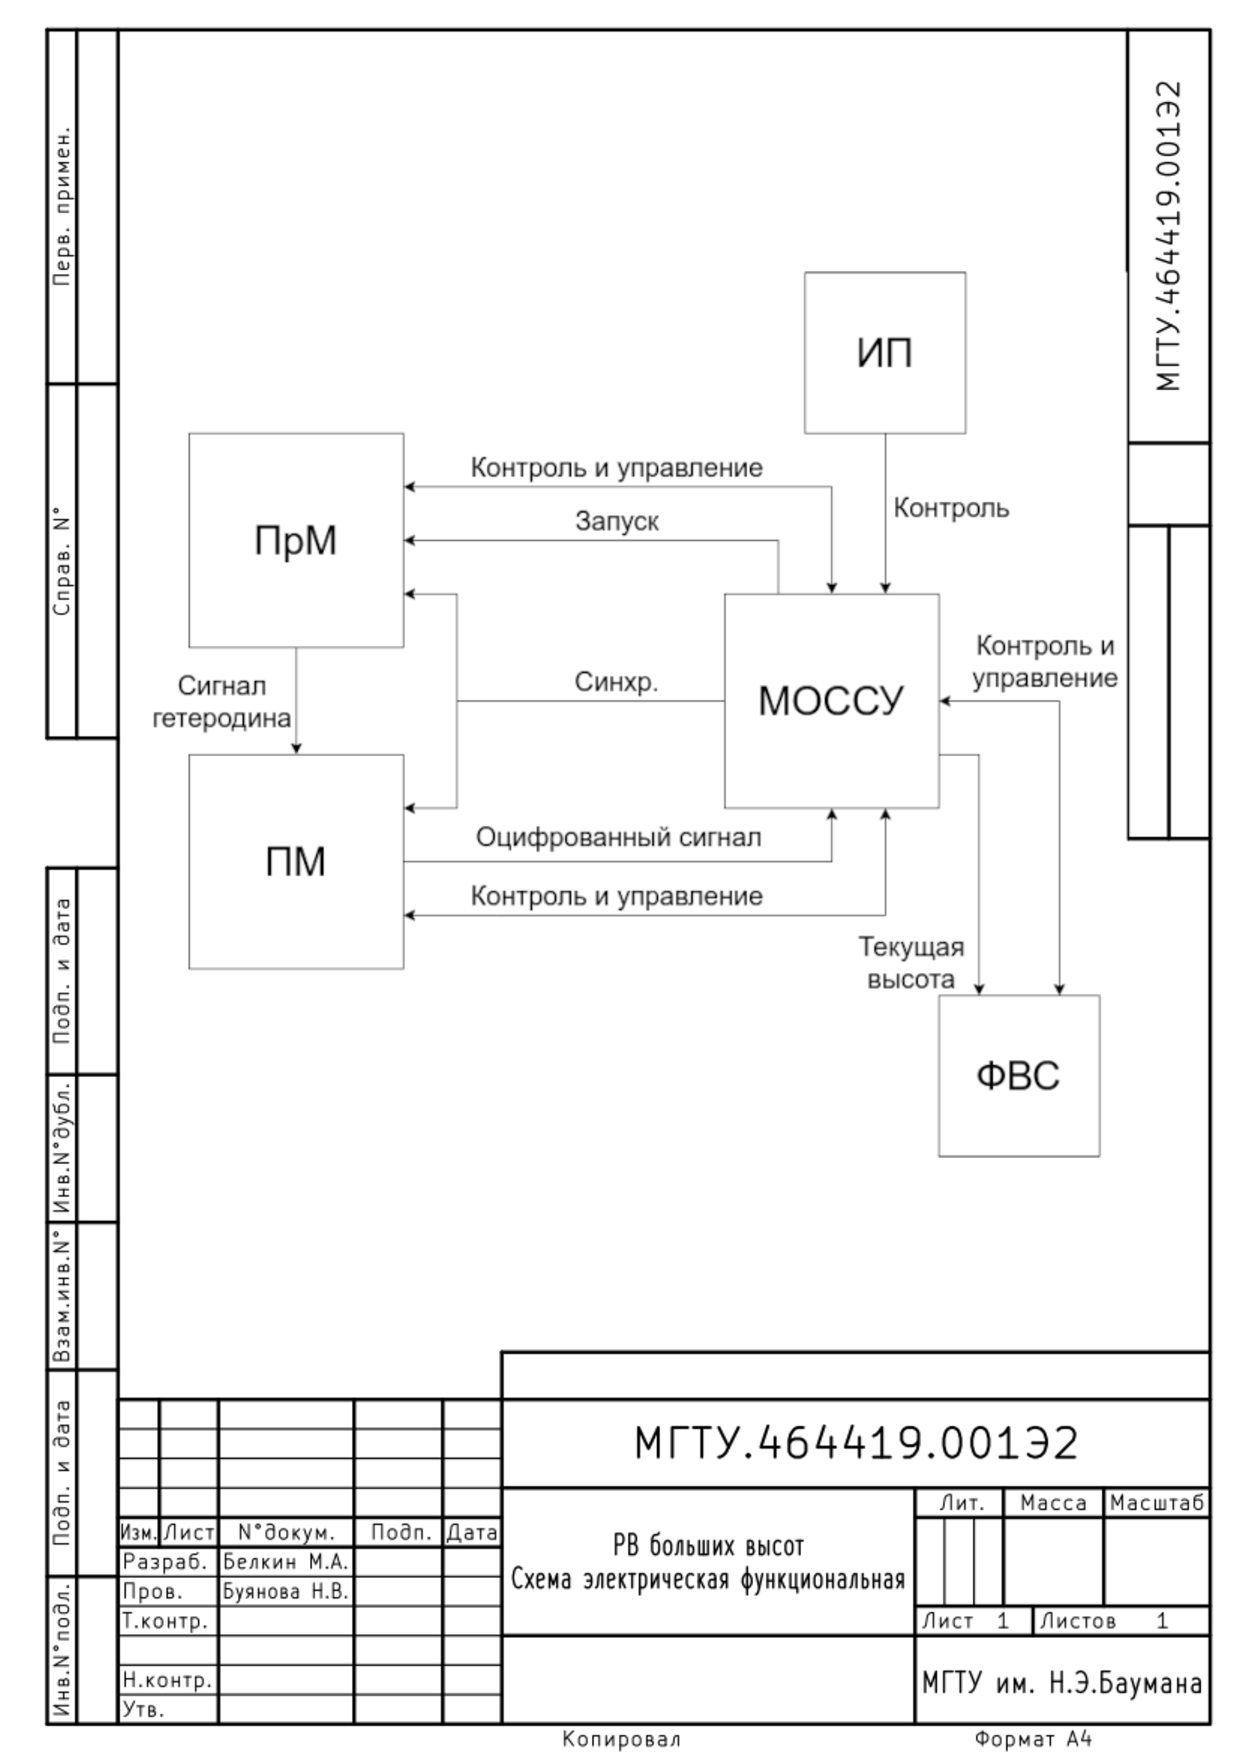
\includepdf[pages=-,fitpaper]{Чертежи/Функциональная схема.pdf}
	\pagebreak
	
	
	\section{S-параметры цепей согласования приёмника}\label{app:receiver_touchstone}
	\pagebreak
	
	\subsection*{Межкаскадная согласующая цепь МШУ}
	\begin{lstlisting}
	#	MHz	S	MA	R	50										
	!	Freq-MHz	S11-mag	S11-arg	S21-mag	S21-arg	S12-mag	S12-arg	S22-mag	S22-arg						
	3000	0.624	-111.19	5.958	94.78	0.105	34.65	0.574	-62.75
	3100	0.640	-114.35	5.926	93.34	0.107	32.91	0.566	-65.29
	3200	0.635	-117.54	5.829	91.86	0.108	31.20	0.553	-67.06
	3300	0.649	-121.01	5.804	90.25	0.109	29.47	0.544	-69.66
	3400	0.643	-123.93	5.714	88.65	0.109	27.91	0.530	-71.45
	3500	0.653	-127.52	5.674	86.88	0.110	26.36	0.519	-73.87
	3600	0.647	-130.30	5.585	85.14	0.110	24.87	0.504	-75.68
	3700	0.653	-133.92	5.544	83.37	0.110	23.66	0.494	-77.96
	3800	0.647	-136.07	5.450	81.68	0.110	22.54	0.481	-79.55
	3900	0.649	-139.89	5.388	79.78	0.110	21.50	0.468	-81.79
	4000	0.647	-141.56	5.304	78.22	0.110	20.58	0.456	-83.35
	4100	0.645	-145.38	5.230	76.33	0.109	19.73	0.444	-85.15
	4200	0.643	-146.69	5.152	74.73	0.110	18.99	0.434	-86.91
	4300	0.642	-150.40	5.080	73.00	0.109	17.85	0.422	-88.99
	4400	0.641	-151.98	5.007	71.28	0.109	17.17	0.412	-90.59
	4500	0.636	-155.56	4.923	69.51	0.108	16.27	0.399	-92.30
	4600	0.638	-156.94	4.854	67.80	0.108	15.62	0.388	-94.18
	4700	0.629	-160.50	4.759	66.08	0.107	14.98	0.376	-95.74
	4800	0.633	-161.39	4.698	64.56	0.106	14.69	0.369	-97.18
	4900	0.621	-165.07	4.601	62.75	0.105	14.20	0.355	-99.00
	5000	0.628	-165.84	4.551	61.25	0.105	14.19	0.351	-100.31
	5200	0.622	-170.00	4.398	58.21	0.104	14.30	0.333	-103.50
	5400	0.618	-173.66	4.257	55.22	0.104	14.17	0.319	-106.32
	5600	0.612	-177.54	4.114	52.29	0.103	14.08	0.304	-109.72
	5800	0.606	179.38	3.983	49.47	0.104	14.70	0.293	-112.40
	6000	0.602	176.14	3.855	46.73	0.105	14.75	0.283	-115.74
	\end{lstlisting}
	%\includepdf[pages=-,fitpaper]{.pdf}
	\pagebreak
	
	
	\subsection*{Согласующая цепь МШУ с антенно-фидерным трактом}
	\begin{lstlisting}
	#	MHz	S	MA	R	50										
	!	Freq-MHz	S11-mag	S11-arg	S21-mag	S21-arg	S12-mag	S12-arg	S22-mag	S22-arg	
	3000  0.748   -73.39  1.301   48.01   0.0195 -130.82   0.89444  -101.35
	3100  0.759   -75.94  1.051   46.93   0.0247 -141.26   0.88926  -106.69
	3200  0.765   -78.22  0.827   48.37   0.0279 -148.72   0.88123  -112.16
	3300  0.777   -80.65  0.638   53.72   0.0330 -155.52   0.86869  -117.06
	3400  0.787   -83.78  0.490   65.45   0.0386 -161.99   0.85269  -122.31
	3500  0.788   -86.66  0.432   84.01   0.0438 -168.22   0.83463  -126.83
	3600  0.797   -89.11  0.449  103.07   0.0490 -173.97   0.81424  -131.68
	3700  0.799   -91.74  0.530  116.92   0.0550 -179.70   0.79412  -136.24
	3800  0.798   -95.10  0.641  122.43   0.0592  173.82   0.76585  -140.42
	3900  0.797   -97.47  0.753  124.53   0.0641  169.70   0.74205  -144.38
	4000  0.797   -99.45  0.860  124.69   0.0672  164.88   0.71366  -148.07
	4100  0.793  -102.26  0.948  122.90   0.0717  161.16   0.68621  -151.18
	4200  0.789  -104.85  1.019  121.25   0.0751  157.40   0.66753  -154.16
	4300  0.786  -106.94  1.095  120.27   0.0797  154.60   0.64865  -157.59
	4400  0.788  -109.00  1.174  118.08   0.0837  149.67   0.62252  -160.92
	4500  0.782  -111.82  1.226  115.60   0.0879  147.18    0.6059  -163.48
	4600  0.778  -114.22  1.294  113.31   0.0954  144.21   0.58487  -166.85
	4700  0.781  -116.19  1.358  111.61   0.1003  142.09   0.56384  -170.24
	4800  0.783  -118.53  1.412  108.91   0.1052  138.55    0.5439  -172.97
	4900  0.775  -121.92  1.481  106.30   0.1115  135.11   0.51845  -176.56
	5000  0.769  -124.13  1.555  103.17   0.1191  131.40   0.48711   179.99
	5100  0.759  -126.27  1.604   99.56   0.1238  127.38   0.45401   177.66
	5200  0.748  -129.29  1.624   95.73   0.1255  123.09   0.42687   176.64
	5300  0.730  -131.14  1.631   92.43   0.1281  119.98    0.4087   176.02
	5400  0.724  -132.14  1.655   89.42   0.1327  117.33   0.38466   174.68
	5500  0.731  -133.96  1.669   87.41   0.1347  115.38   0.37072   172.66
	5600  0.713  -137.30  1.679   83.99   0.1377  111.76   0.35235   171.92
	5700  0.692  -139.18  1.693   80.87   0.1424  109.58   0.33155   171.80
	5800  0.707  -139.20  1.720   78.96   0.1466  107.33   0.31087   170.75
	5900  0.706  -142.70  1.695   75.52   0.1461  104.30    0.2935   171.73
	6000  0.637  -145.48  1.636   71.63   0.1436  100.43   0.29168   174.71
	\end{lstlisting}
	\pagebreak
	
	
	\subsection*{Согласующая цепь МШУ со смесителем}
	\begin{lstlisting}
	#	MHz	S	MA	R	50										
	!	Freq-MHz	S11-mag	S11-arg	S21-mag	S21-arg	S12-mag	S12-arg	S22-mag	S22-arg	
	3000  0.451   -50.350	2.598	66.130	0.068	45.820	0.719	-62.230
	3100  0.466   -51.710	2.399	62.200	0.066	41.740	0.732	-68.010
	3200  0.481   -53.320	2.208	58.650	0.063	37.720	0.742	-73.690
	3300  0.497   -55.100	2.025	55.520	0.060	33.860	0.752	-79.240
	3400  0.511   -57.250	1.854	52.660	0.057	30.030	0.760	-84.720
	3500  0.524   -59.460	1.689	50.220	0.053	26.370	0.765	-90.150
	3600  0.538   -61.890	1.535	48.300	0.049	22.770	0.767	-95.560
	3700  0.551   -64.610	1.390	47.080	0.045	19.510	0.769	-100.88
	3800  0.564   -67.420	1.259	46.610	0.040	16.930	0.770	-106.10
	3900  0.576   -70.400	1.141	47.010	0.035	14.410	0.769	-111.30
	4000  0.587   -73.450	1.039	48.390	0.029	12.690	0.765	-116.49
	4100  0.597   -76.590	0.954	50.740	0.023	12.590	0.760	-121.64
	4200  0.605   -79.930	0.892	54.110	0.017	16.670	0.753	-126.67
	4300  0.613   -83.350	0.854	58.060	0.012	29.940	0.747	-131.55
	4400  0.620   -86.710	0.838	62.280	0.008	62.470	0.738	-136.38
	4500  0.627   -90.330	0.842	65.990	0.010	103.250	0.728	-141.18
	4600  0.632   -94.080	0.862	69.170	0.016	121.230	0.716	-145.85
	4700  0.636   -97.870	0.899	71.380	0.024	126.390	0.704	-150.33
	4800  0.639   -101.630	0.944	72.590	0.032	127.070	0.692	-154.65
	4900  0.639   -105.400	0.994	72.810	0.040	125.910	0.679	-158.85
	5000  0.639   -109.350	1.043	72.120	0.048	123.350	0.665	-162.90
	5100  0.636   -113.210	1.088	70.880	0.056	120.240	0.651	-166.74
	5200  0.632   -117.030	1.131	69.210	0.063	116.850	0.639	-170.33
	5300  0.628   -120.520	1.173	67.160	0.070	113.540	0.629	-173.80
	5400  0.627   -124.180	1.207	64.760	0.077	110.810	0.617	-177.19
	5500  0.624   -127.930	1.236	62.300	0.085	107.900	0.605	179.570
	5600  0.621   -131.700	1.265	59.580	0.092	104.650	0.595	176.540
	5700  0.617   -135.620	1.288	56.530	0.099	101.340	0.587	173.730
	5800  0.610   -139.410	1.304	53.480	0.105	98.050	0.580	171.050
	5900  0.603   -143.140	1.313	50.400	0.112	94.950	0.573	168.440
	6000  0.597   -146.730	1.319	47.320	0.118	91.360	0.567	165.990
	\end{lstlisting}
	\pagebreak
	
	
	\subsection*{Согласующая цепь усилителя сигнала гетеродина со смесителем}
	\begin{lstlisting}
	#	MHz	S	MA	R	50										
	!	Freq-MHz	S11-mag	S11-arg	S21-mag	S21-arg	S12-mag	S12-arg	S22-mag	S22-arg	
	3000   0.90874   -78.55   0.179   33.34   0.179   33.05   0.939  -40.47
	3100   0.91285   -80.34   0.183   31.89   0.184   31.62   0.937  -41.85
	3200   0.90369   -83.32   0.186   29.83   0.187   29.52   0.934  -43.25
	3300   0.90908   -85.11   0.191   28.35   0.197   28.04   0.932  -44.67
	3400   0.90036   -88.02   0.193   26.37   0.194   26.02   0.930  -46.04
	3500   0.90543   -89.89   0.197   24.75   0.191   24.39   0.927  -47.51
	3600    0.8963   -92.79   0.199   22.74   0.200   22.31   0.924  -48.98
	3700   0.90163   -94.51   0.203   21.34   0.203   20.97   0.923  -50.36
	3800   0.89309   -97.28   0.205   19.45   0.205   19.04   0.920  -51.79
	3900   0.89758   -99.28   0.208   17.83   0.208   17.44   0.916  -53.34
	4000   0.88921  -101.70   0.210   16.08   0.210   15.73   0.914  -54.76
	4100   0.89336  -104.03   0.212   14.38   0.213   13.96   0.912  -56.24
	4200   0.88491  -106.16   0.214   12.87   0.219   12.51   0.909  -57.76
	4300   0.88943  -108.33   0.217   11.08   0.217   10.61   0.907  -59.24
	4400   0.88422  -110.59   0.218    9.31   0.218    8.89   0.909  -60.71
	4500   0.88751  -112.86   0.220    7.46   0.220    6.96   0.901  -62.22
	4600   0.88215  -115.05   0.223    5.64   0.221    5.18   0.899  -63.90
	4700    0.8861  -117.30   0.222    3.85   0.222    3.26   0.898  -65.46
	4800   0.88066  -119.37   0.222    2.19   0.222    1.65   0.895  -66.97
	4900   0.88477  -121.74   0.222    0.28   0.222   -0.30   0.892  -68.53
	5000   0.88015  -123.59   0.223   -1.36   0.222   -1.86   0.890  -70.33
	5200   0.87811  -127.98   0.228   -4.61   0.221   -5.06   0.886  -73.63
	5400   0.87608  -132.23   0.221   -7.79   0.220   -8.29   0.879  -76.93
	5600   0.87586  -136.62   0.218  -11.54   0.217  -12.01   0.876  -80.57
	5800   0.87318  -140.78   0.215  -14.52   0.214  -15.04   0.870  -83.99
	6000   0.87082  -144.91   0.212  -17.72   0.214  -18.21   0.865  -87.84
	\end{lstlisting}
	\pagebreak
	
	
%	\subsection*{Согласующая цепь гетеродина со смесителем}
%	\begin{lstlisting}
%	#	MHz	S	MA	R	50										
%	!	Freq-MHz	S11-mag	S11-arg	S21-mag	S21-arg	S12-mag	S12-arg	S22-mag	S22-arg	
%	3000  0.736   -77.21   1.249    46.88  0.018  -119.94   0.8895  -101.46
%	3100  0.747   -79.70   1.009    45.85  0.029  -128.06   0.8839  -106.85
%	3200  0.756   -81.80   0.795    47.25  0.024  -138.11   0.8751  -112.28
%	3300  0.768   -84.08   0.615    52.62  0.031  -145.96    0.862  -117.21
%	3400  0.780   -87.20   0.475    64.33  0.036  -153.84   0.8468  -122.42
%	3500  0.785   -89.96   0.419    82.89  0.040  -160.41   0.8283  -127.11
%	3600  0.793   -92.22   0.437   101.87  0.046  -166.22   0.8087  -132.04
%	3700  0.797   -94.79   0.519   115.60  0.050  -172.98   0.7870  -136.63
%	3800  0.797   -97.98   0.630   120.93  0.055  -178.40     0.75  -140.91
%	3900  0.799  -100.35   0.739   122.89  0.008   175.71   0.7336  -144.97
%	4000  0.800  -102.42   0.847   122.74  0.065   170.74   0.7055  -148.67
%	4100  0.800  -105.17   0.932   120.84  0.066   165.71   0.6774  -151.97
%	4200  0.796  -107.78   0.999   119.09  0.070   162.87   0.6585  -154.94
%	4300  0.799  -109.58   1.077   118.12  0.075   159.63   0.6385  -158.43
%	4400  0.800  -111.63   1.155   115.80  0.080   156.71   0.6113  -161.84
%	4500  0.799  -114.43   1.208   113.11  0.084   152.81   0.5930  -164.40
%	4600  0.797  -117.00   1.275   110.79  0.087   149.35    0.571  -167.87
%	4700  0.802  -118.67   1.342   108.94  0.094   147.09   0.5504  -171.40
%	4800  0.804  -121.26   1.397   106.23  0.099   144.22   0.5277  -174.45
%	4900  0.799  -124.54   1.465   103.42  0.106   140.50   0.5018  -178.08
%	5000  0.794  -126.66   1.541   100.12  0.114   136.14    0.468   178.12
%	5100  0.787  -128.79   1.591    96.37  0.119   131.51   0.4322   175.93
%	5200  0.777  -131.75   1.613    92.39  0.121   127.25   0.4038   175.03
%	5300  0.762  -133.63   1.620    88.91  0.123   124.34    0.383   174.48
%	5400  0.756  -134.68   1.642    85.84  0.127   121.94   0.3595   173.13
%	5500  0.764  -136.27   1.656    83.75  0.130   119.83   0.3446   170.75
%	5600  0.747  -139.63   1.669    80.15  0.132   116.66   0.3226   170.47
%	5700  0.729  -141.74   1.683    76.89  0.137   113.74   0.3014   170.61
%	5800  0.745  -141.66   1.711    74.84  0.141   112.09   0.2805   169.76
%	5900  0.745  -144.84   1.685    71.36  0.142   107.79   0.2601   171.65
%	6000  0.673  -147.94   1.625    67.30  0.138   105.51   0.2608   175.35
%	\end{lstlisting}
%	\pagebreak
	
	
%	\subsection*{Межкаскадная согласующая цепь МШУ}
%	\begin{lstlisting}
%	#	MHz	S	MA	R	50										
%	!	Freq-MHz	S11-mag	S11-arg	S21-mag	S21-arg	S12-mag	S12-arg	S22-mag	S22-arg	
%		
%	\end{lstlisting}
%	\pagebreak
	
	
	
	\section{Схемы модуля приёмника}\label{app:receiver}
	\pagebreak
%	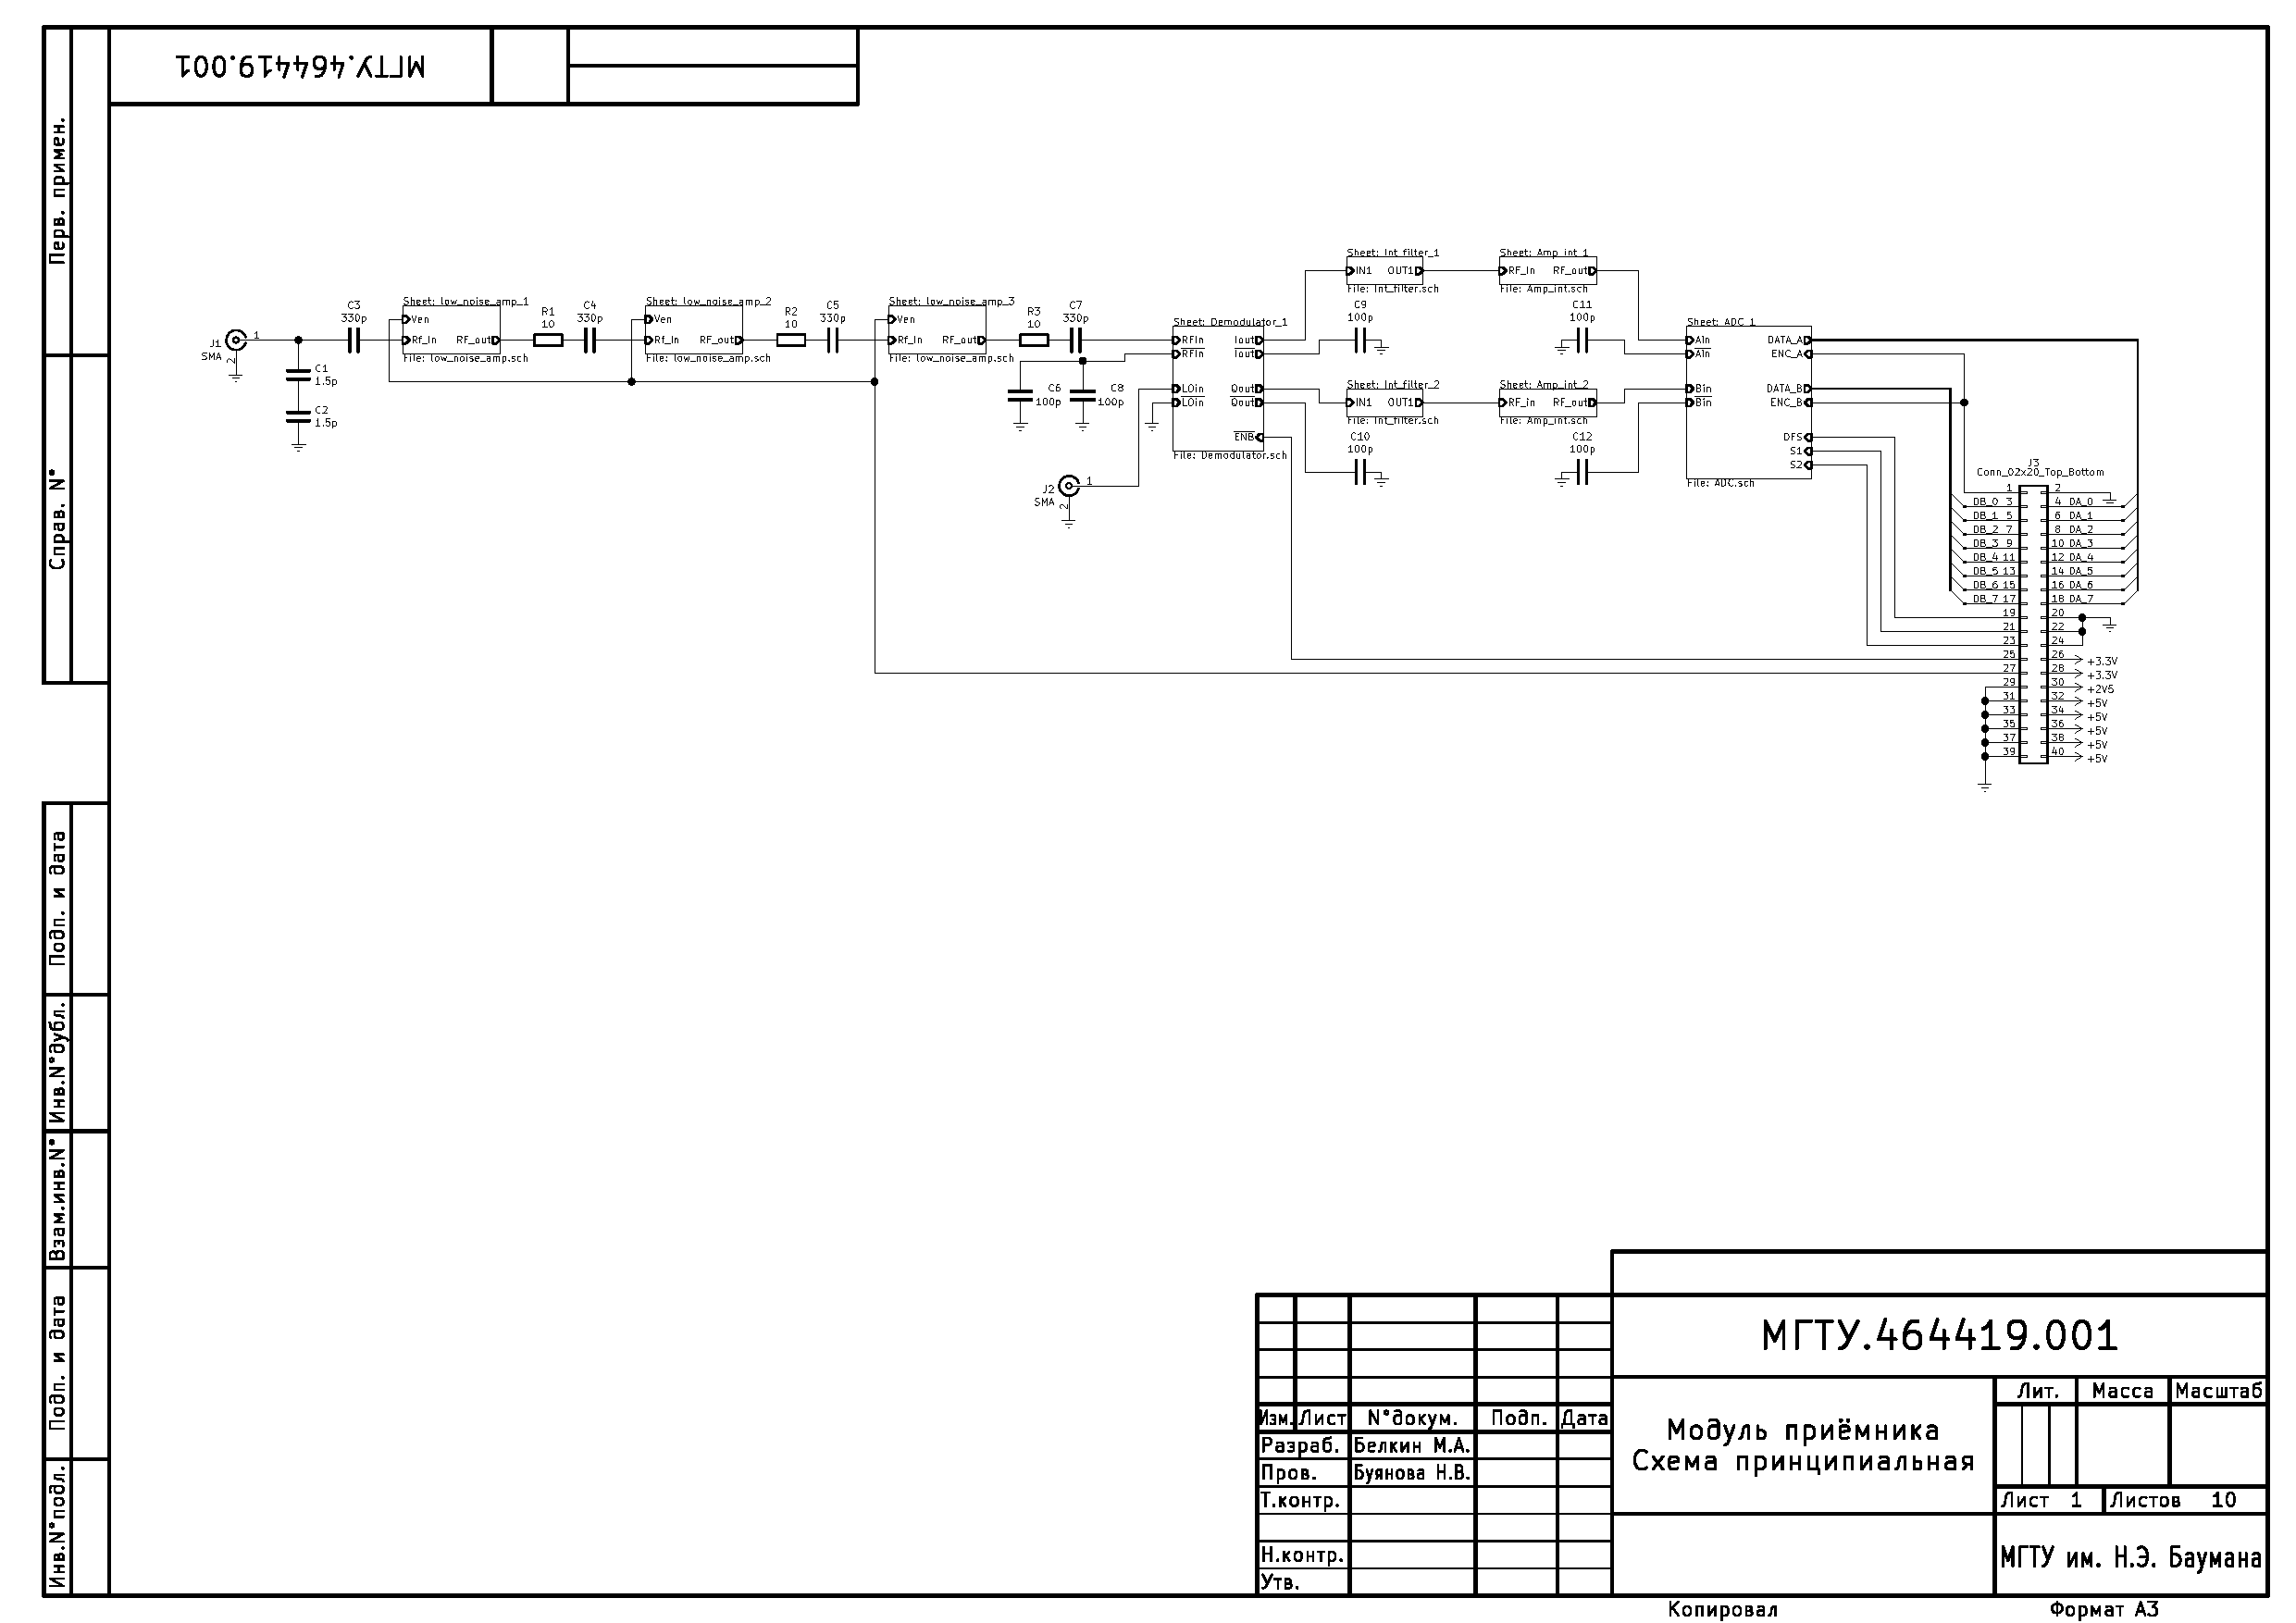
\includepdf[landscape=true,pages=-,fitpaper]{Чертежи/ПриёмникТитульный.pdf}
%	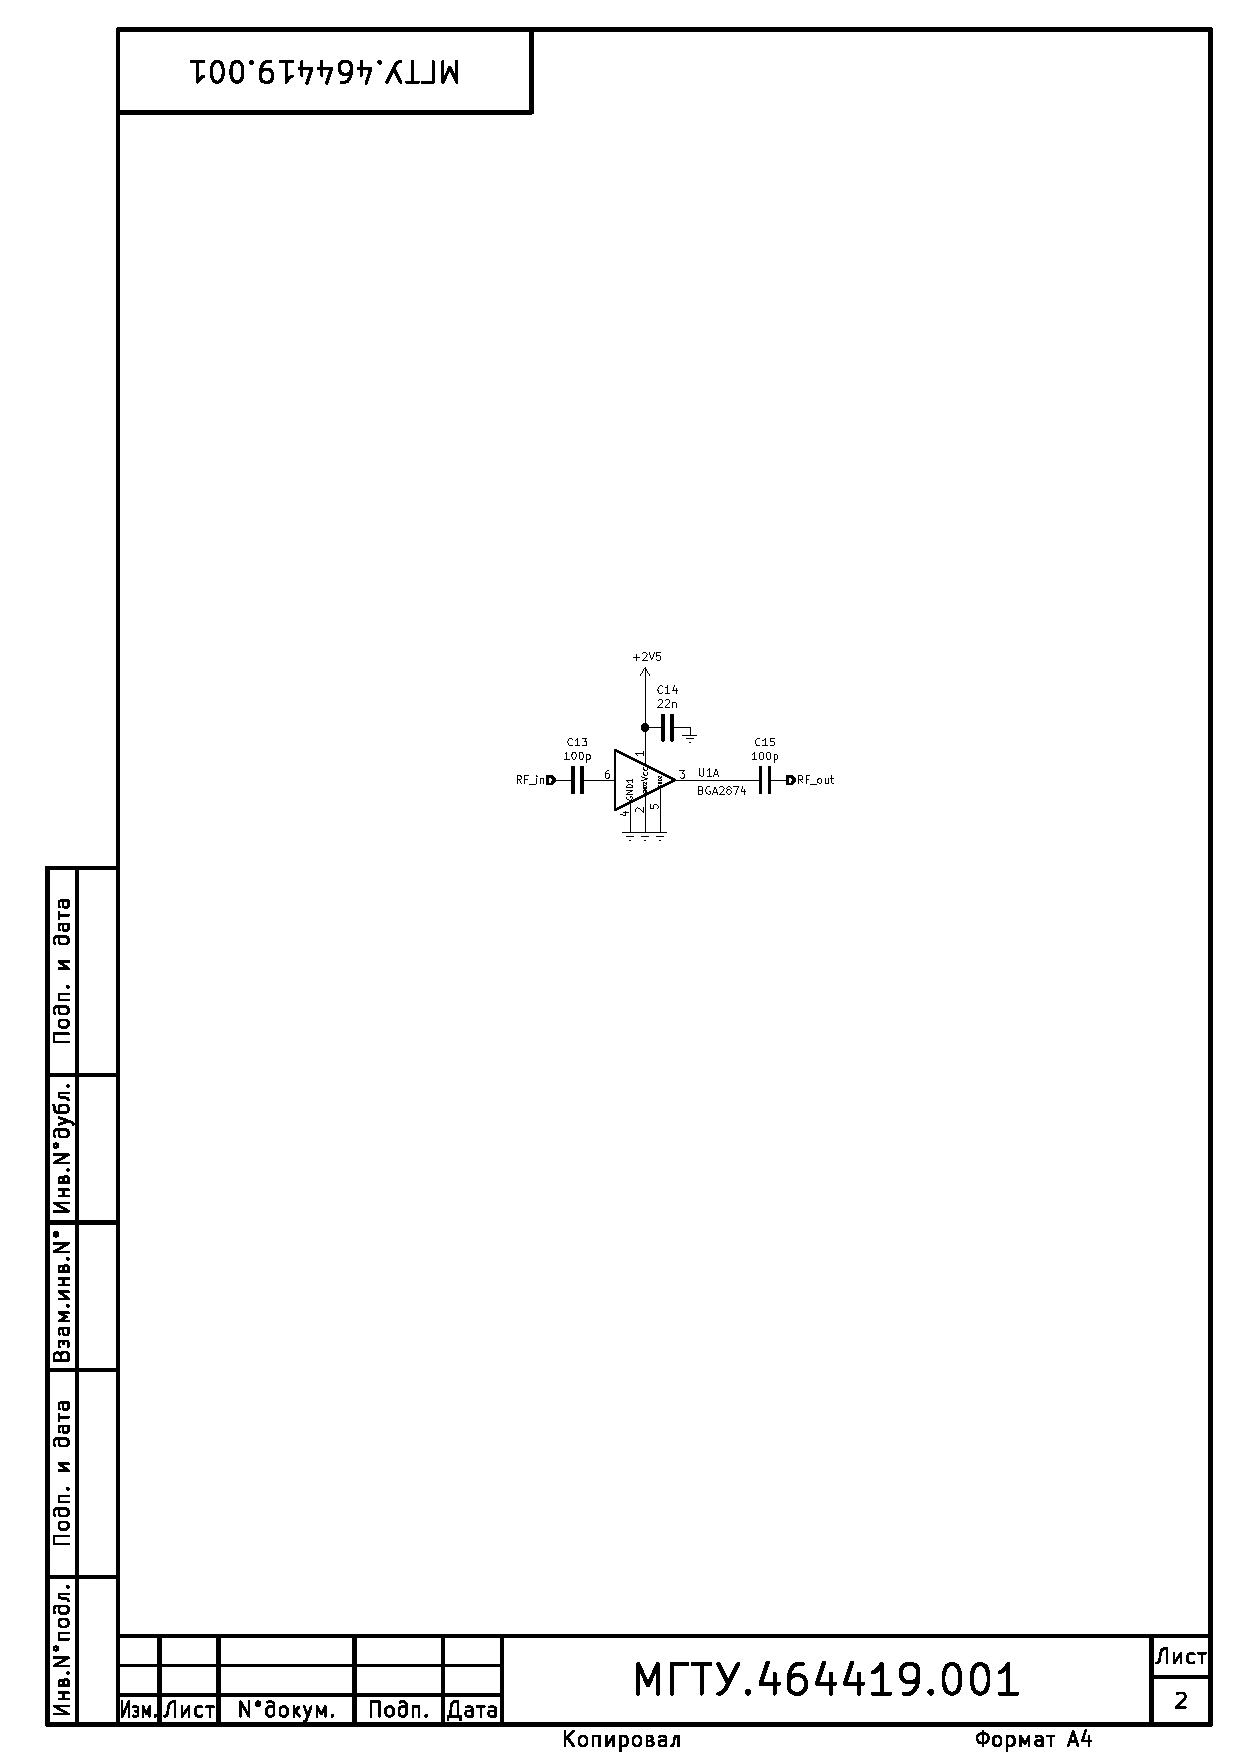
\includepdf[pages=-]{Чертежи/ПриёмникВторичные.pdf}
	\pagebreak
	

	
	
	

\end{document}